\documentclass{beamer}
\usepackage{tikz}
\usepackage[all]{xy}
\usepackage{amsmath,amssymb}
\usepackage{hyperref}
\usepackage{graphicx}
 
\DeclareMathOperator*{\argmin}{arg\,min}
\DeclareMathOperator*{\Lik}{Lik}
\DeclareMathOperator*{\PoissonLoss}{PoissonLoss}
\DeclareMathOperator*{\Peaks}{Peaks}
\DeclareMathOperator*{\Segments}{Segments}
\DeclareMathOperator*{\argmax}{arg\,max}
\DeclareMathOperator*{\maximize}{maximize}
\DeclareMathOperator*{\minimize}{minimize}
\newcommand{\sign}{\operatorname{sign}}
\newcommand{\RR}{\mathbb R}
\newcommand{\ZZ}{\mathbb Z}
\newcommand{\NN}{\mathbb N}
\newcommand{\z}{$z = 2, 4, 3, 5, 1$} 

\newcommand{\algo}[1]{\textcolor{#1}{#1}}
\definecolor{PDPA}{HTML}{66C2A5}
\definecolor{CDPA}{HTML}{FC8D62}
\definecolor{GPDPA}{HTML}{4D4D4D}

% Set transparency of non-highlighted sections in the table of
% contents slide.
\setbeamertemplate{section in toc shaded}[default][100]
\AtBeginSection[]
{
  \setbeamercolor{section in toc}{fg=red} 
  \setbeamercolor{section in toc shaded}{fg=black} 
  \begin{frame}
    \tableofcontents[currentsection]
  \end{frame}
}

\begin{document}

\title{Introduction to deep learning in R}

\author{
  Toby Dylan Hocking\\
  toby.hocking@nau.edu\\
  toby.hocking@r-project.org\\
}

\maketitle

\section{Introduction and overview}

\begin{frame}
  \frametitle{Machine learning intro: image classification example}
  ML is all about learning predictive functions $f(x)\approx y$, where 
  \begin{itemize}
  \item Inputs/features $x$ can be easily computed using traditional
    algorithms. For example, matrix of pixel intensities in an image.
  \item Outputs/labels $y$ are what we want to predict, typically more
    difficult/costly to measure than inputs. For example, to get an
    image class label, you may have to ask a human. 
  \item Input $x$ = image of digit, output $y\in\{0,1,\dots,9\}$, \\--
    this is a classification problem with 10 classes.\\
  $f(
\includegraphics[height=1cm]{mnist-0})=0$,
  $f(
\includegraphics[height=1cm]{mnist-1})=1$
\item Traditional/unsupervised algorithm: I give you a pixel intensity matrix
  $x\in\RR^{28\times 28}$, you code a function $f$ that returns one of
  the 10 possible digits. Q: how to do that?
  \end{itemize}
\end{frame}

\begin{frame}
  \frametitle{Supervised machine learning algorithms}

  I give you a training data set with paired inputs/outputs, e.g.

  \begin{center}
    \Huge 0 1 2 3 4 5 6 7 8 9

  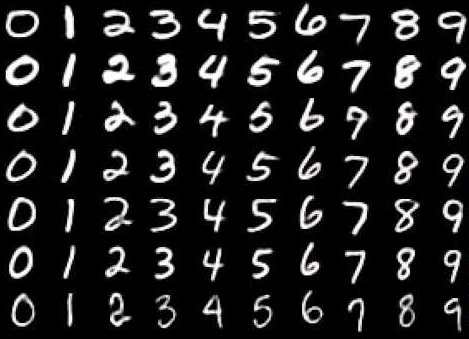
\includegraphics[height=1.9in]{mnist-digits}
  \end{center}

  Your job is to code an algorithm, \textsc{Learn}, that infers a
  function $f$ from the training data. (you don't code $f$)
  
  \scriptsize Source: github.com/cazala/mnist
\end{frame}


\begin{frame}
  \frametitle{Advantages of supervised machine learning}

  \begin{center}
    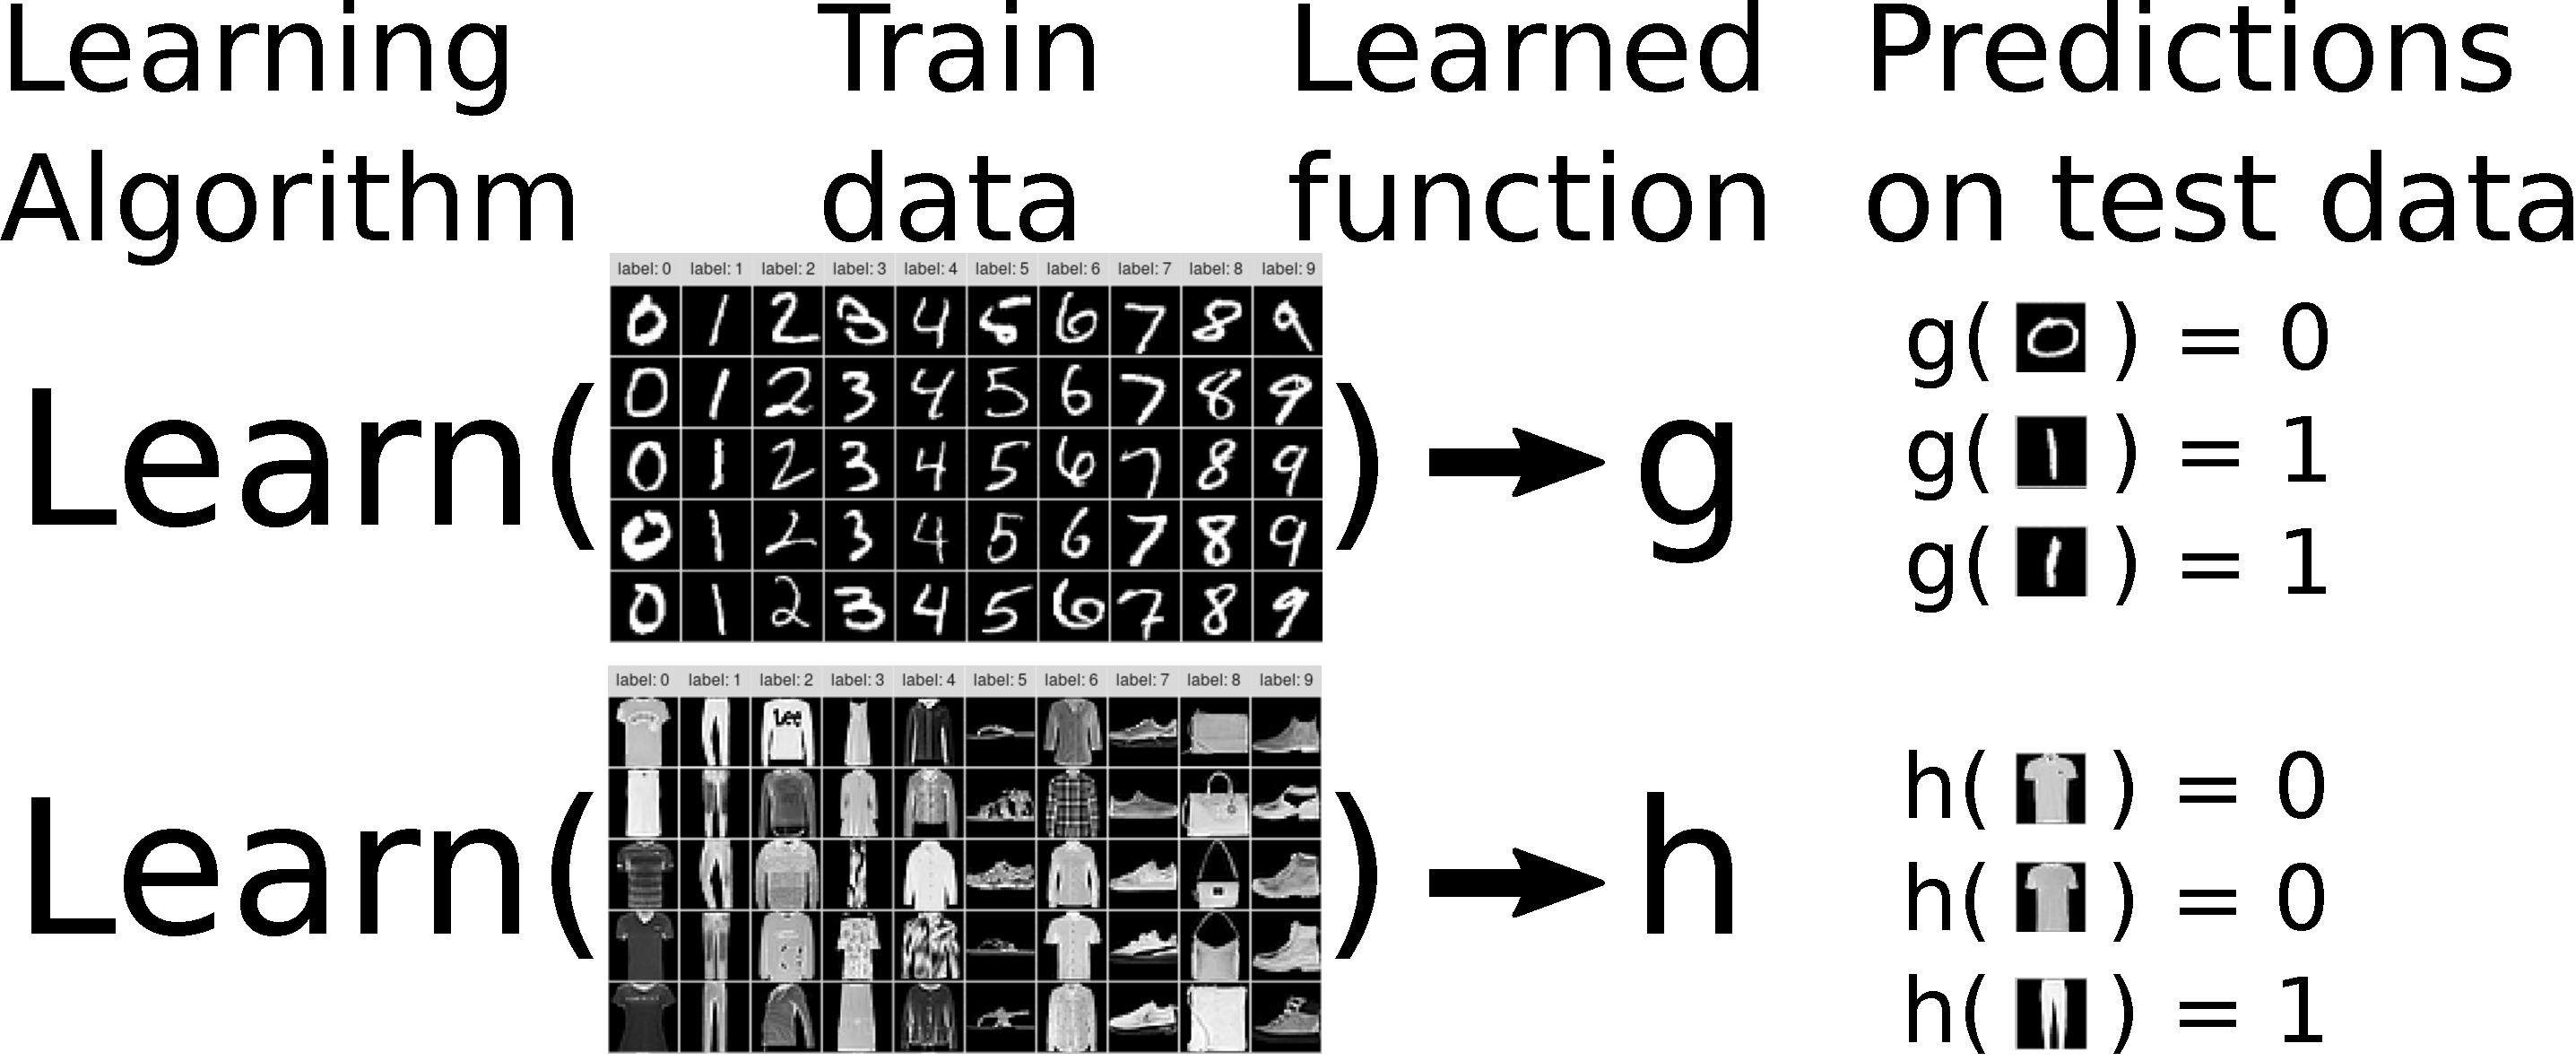
\includegraphics[width=0.8\textwidth]{drawing-mnist-train-test.pdf}
  \end{center}
  \vskip -0.2cm
  
  \begin{itemize}
  \item Input $x\in\RR^{28\times 28}$, output $y\in\{0,1,\dots,9\}$
    types the same!
  \item Can use same learning algorithm regardless of pattern.
  \item Pattern encoded in the labels (not the algorithm).
  \item Useful if there are many un-labeled data, but few labeled data
    (or getting labels is long/costly).
  \item State-of-the-art accuracy (if there is enough training data).
  \end{itemize}

  \scriptsize Sources: github.com/cazala/mnist, github.com/zalandoresearch/fashion-mnist

\end{frame}

\begin{frame}
  \frametitle{Overview of tutorial}
  In this tutorial we will discuss two kinds of problems, which
  differ by the type of the output/label/y variable we want to predict.
  \begin{itemize}
  \item Regression, y is a real number.
  \item Classification, y is an integer representing a category.
  \end{itemize}

  The rest of the tutorial will focus on three examples:
  \begin{enumerate}
  \item Regression with a single input, to demonstrate how to avoid
    overfitting.
  \item Classification of digit images, to demonstrate how to compare
    machine learning algorithms in terms of test/prediction accuracy.
  \end{enumerate}
\end{frame}

\section{Example 1: avoiding overfitting in regression, overview of concepts
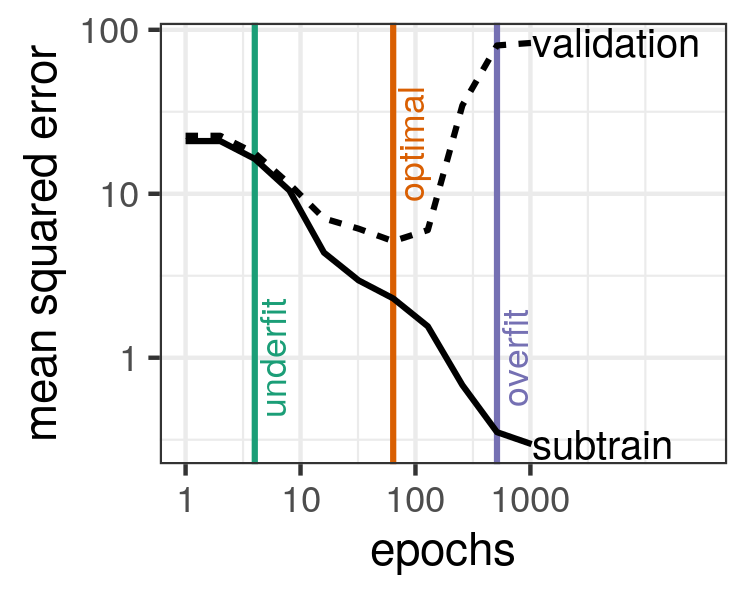
\includegraphics[height=3cm]{figure-overfitting-paper-loss}}   
 
\begin{frame}
  \frametitle{Goal of this section: demonstrate how to avoid
    overfitting}
  \begin{itemize}
  \item The goal of supervised machine learning is to get accurate
    predictions on new/unseen/held-out test data.
  \item The data used during learning are caled the train set.
  \item Any machine learning algorithm is prone to overfit, which
    means providing better predictions on the train set than
    on a held-out validation/test set. (BAD)
  \item To learn a model which does NOT overfit (GOOD), you need to
    divide your train set into subtrain/validation sets (subtrain used
    as input to gradient descent algorithm, validation set used to
    control number of iterations of gradient descent).
  \item Code for figures in this section:
    \url{https://github.com/tdhock/2023-res-baz-az/blob/main/figure-overfitting.R}
  \end{itemize}
\end{frame}

\begin{frame}
  \frametitle{Three different data sets/patterns}
  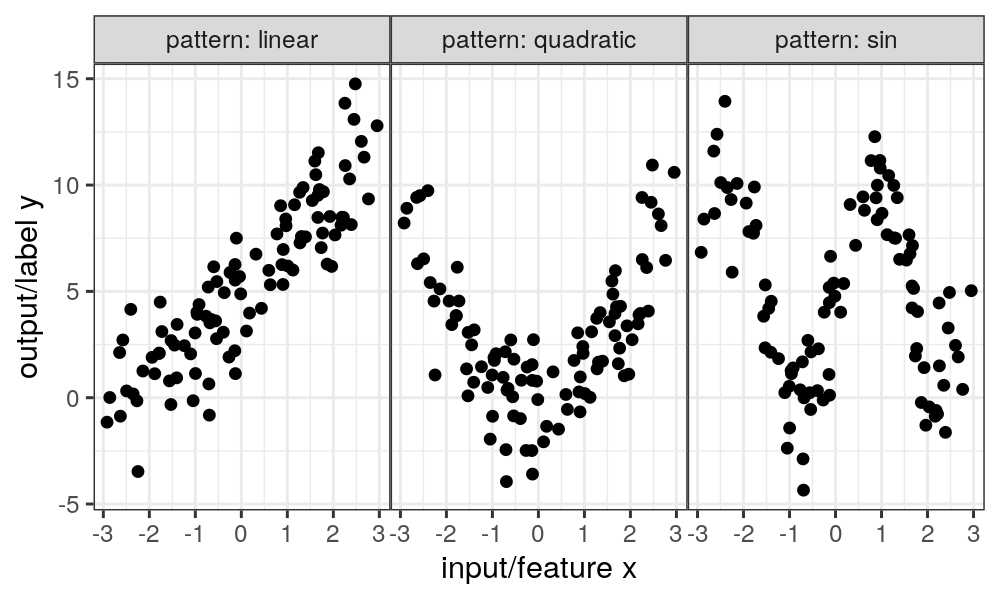
\includegraphics[width=\textwidth]{figure-overfitting-data}

  \begin{itemize}
   \item We illustrate this using a single input/feature
    $x\in\mathbb R$.
  \item We use a regression problem with outputs $y\in\mathbb R$.
  \item Goal is to learn a function $f(x)\in\mathbb R$.
  \end{itemize}
\end{frame}

\begin{frame}
  \frametitle{K-fold cross-validation for splitting data}
  \begin{itemize}
  \item One way to split is via K-fold cross-validation. 
\item Each row is assigned a fold ID number from 1 to K.
\item For each for ID, those data are held out, and other data are kept.
\item Popular relative to other splitting methods because of simplicity and fairness (each row is held out one time).
\end{itemize}
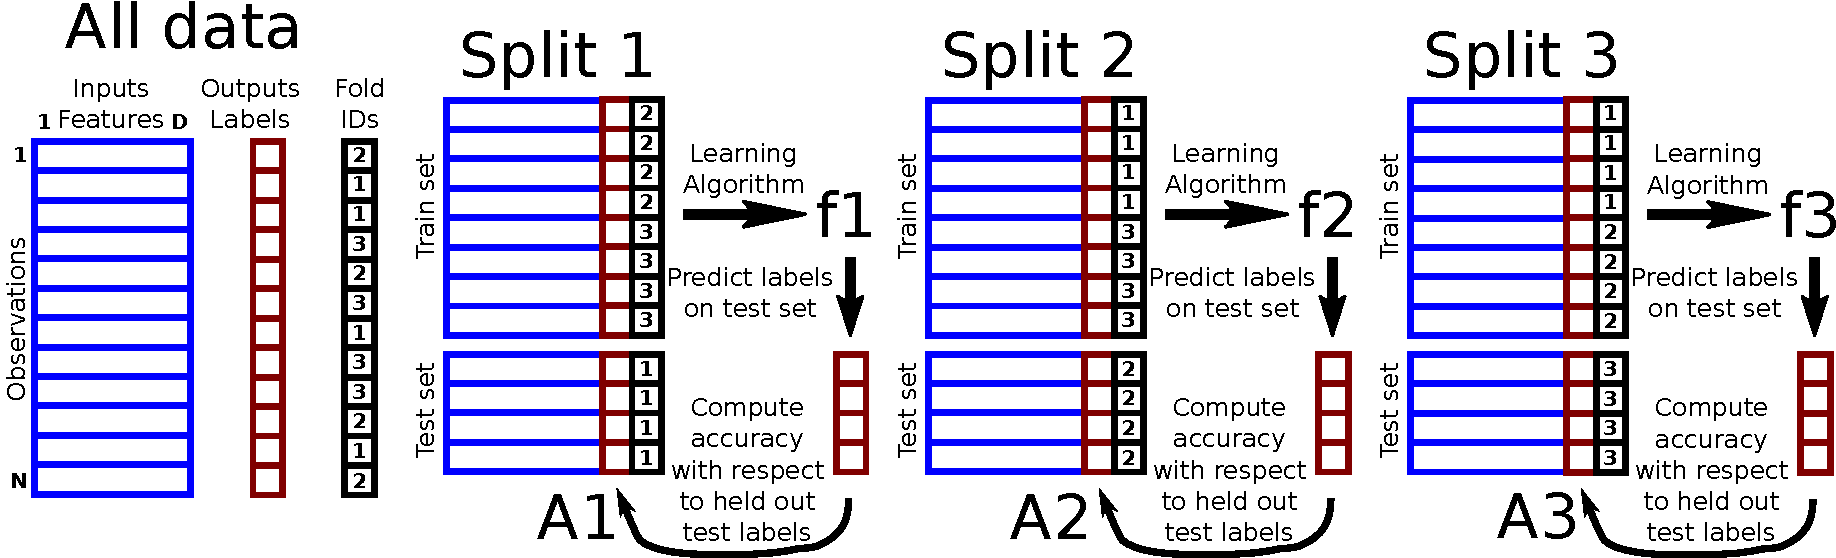
\includegraphics[width=\textwidth]{drawing-cross-validation}
\end{frame}

\begin{frame}
  \frametitle{Illustration of 4-fold cross-validation}
  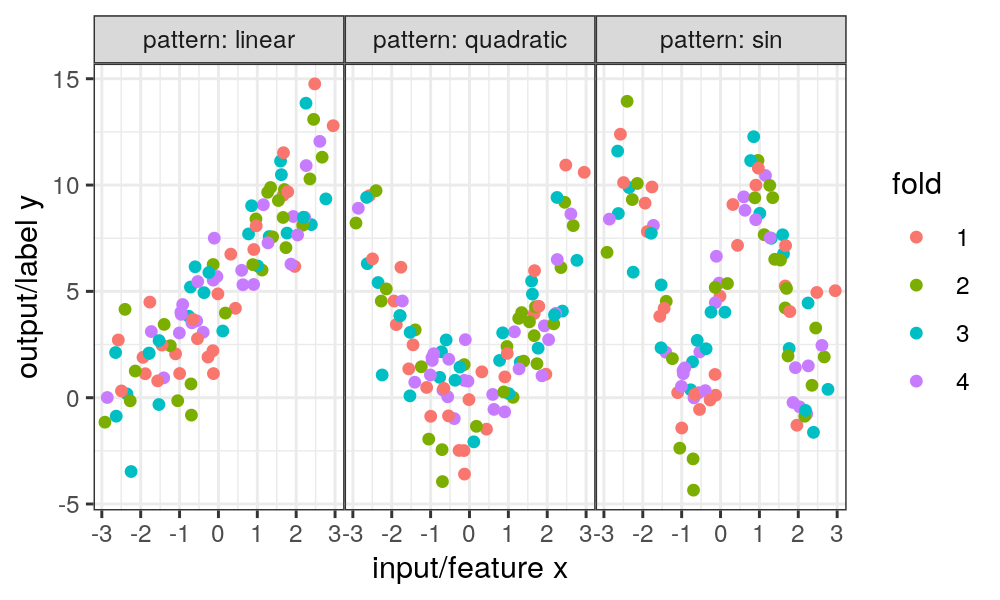
\includegraphics[width=\textwidth]{figure-overfitting-data-folds}

  Randomly assign each observation a fold ID from 1 to 4.
  
\end{frame}

\begin{frame}
  \frametitle{Neural network learning algorithm}
  \begin{itemize}
  \item We will fit a neural network to these data.
  \item The neural network learns how to predict the outputs from the inputs.
  \item The learning algorithm is gradient descent, which iteratively
    minimizes the loss of the predictions with respect to the labels
    in the subtrain set.
  \item We also compute the loss on the validation set, so we can
    select the number of gradient descent iterations that gives the
    best predictions on new data (avoiding overfitting).
  \end{itemize}
\end{frame}
 
\begin{frame}
  \frametitle{Illustration of subtrain/validation split}
  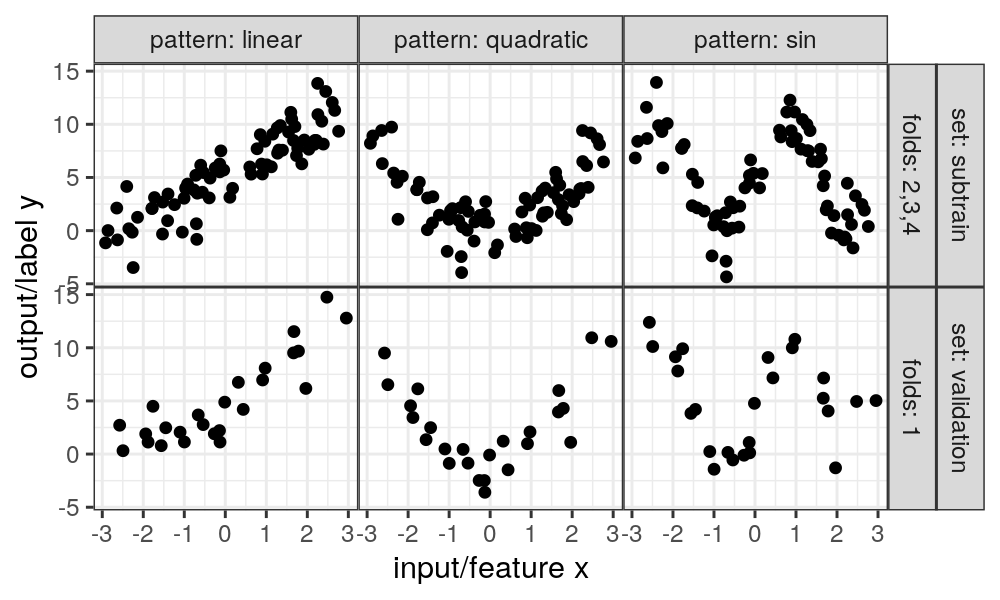
\includegraphics[width=\textwidth]{figure-overfitting-data-sets}

  \begin{itemize}
  \item For validation fold 1, all observations with that fold ID are
    considered the validation set.
  \item All other observations are considered the subtrain set.
  \end{itemize}
\end{frame}


\begin{frame}
  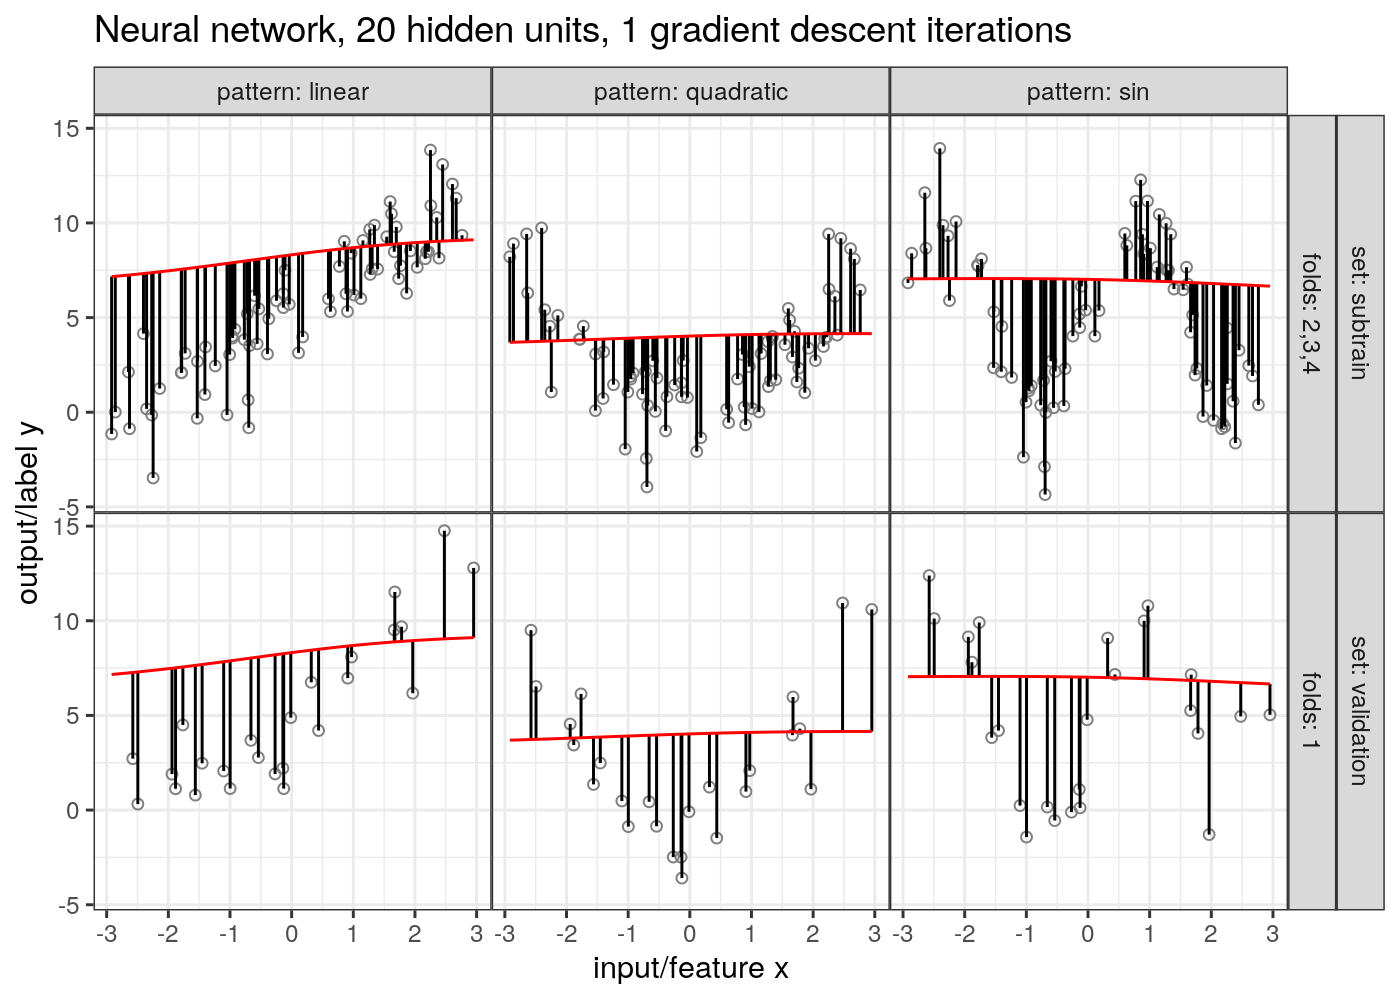
\includegraphics[width=\textwidth]{figure-overfitting-pred-units=20-maxit=1.png}
\
Data=grey dots, predictions=red curve, loss=black vertical line segments.
\end{frame}


\begin{frame}
  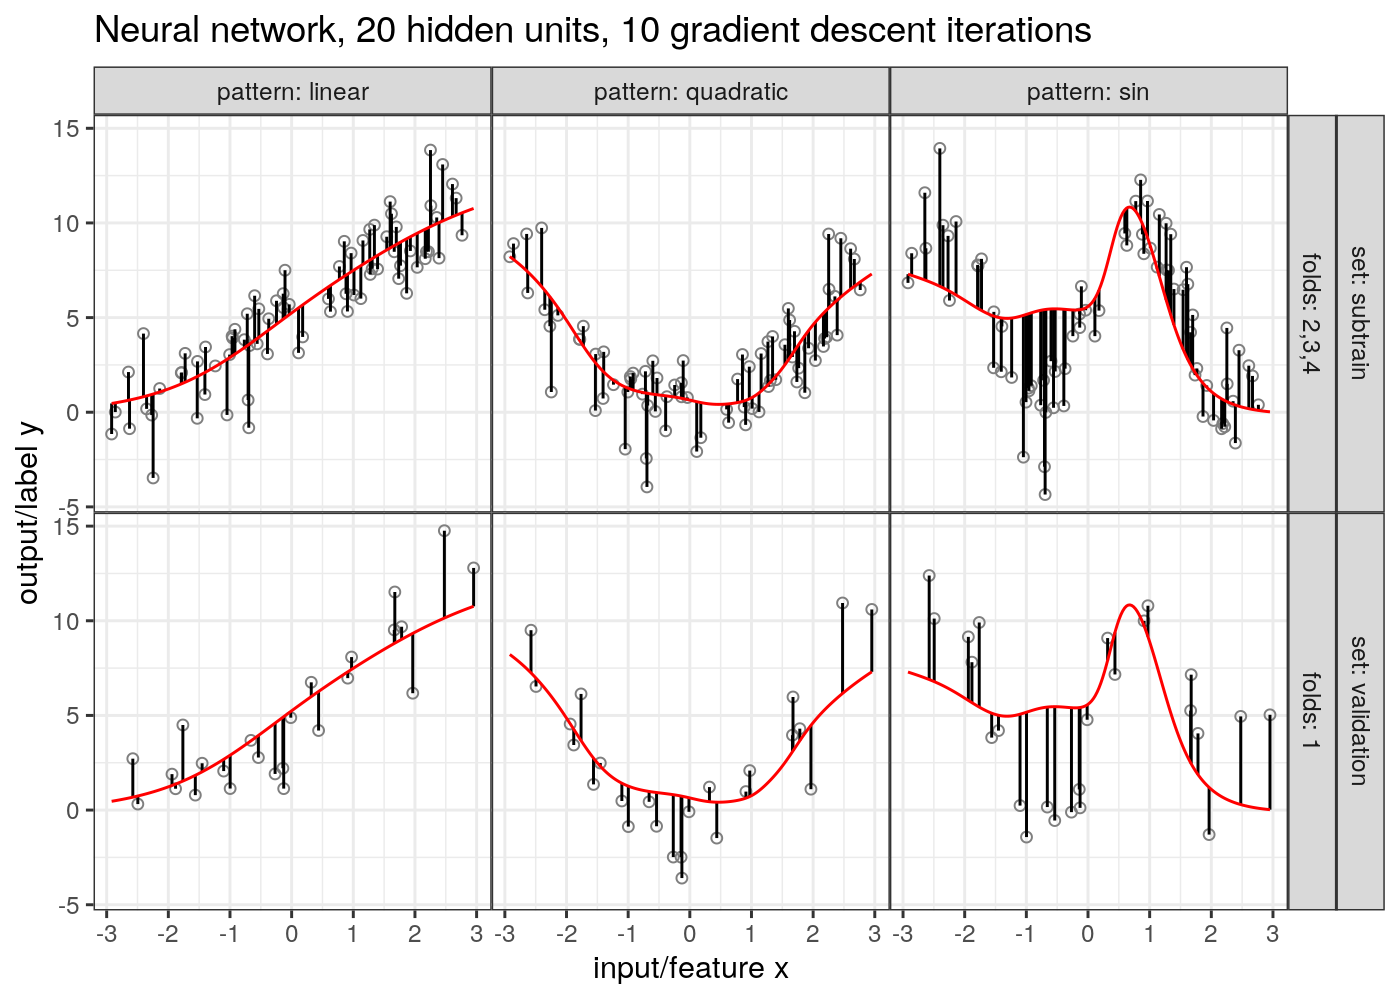
\includegraphics[width=\textwidth]{figure-overfitting-pred-units=20-maxit=10.png}
\
Data=grey dots, predictions=red curve, loss=black vertical line segments.
\end{frame}


\begin{frame}
  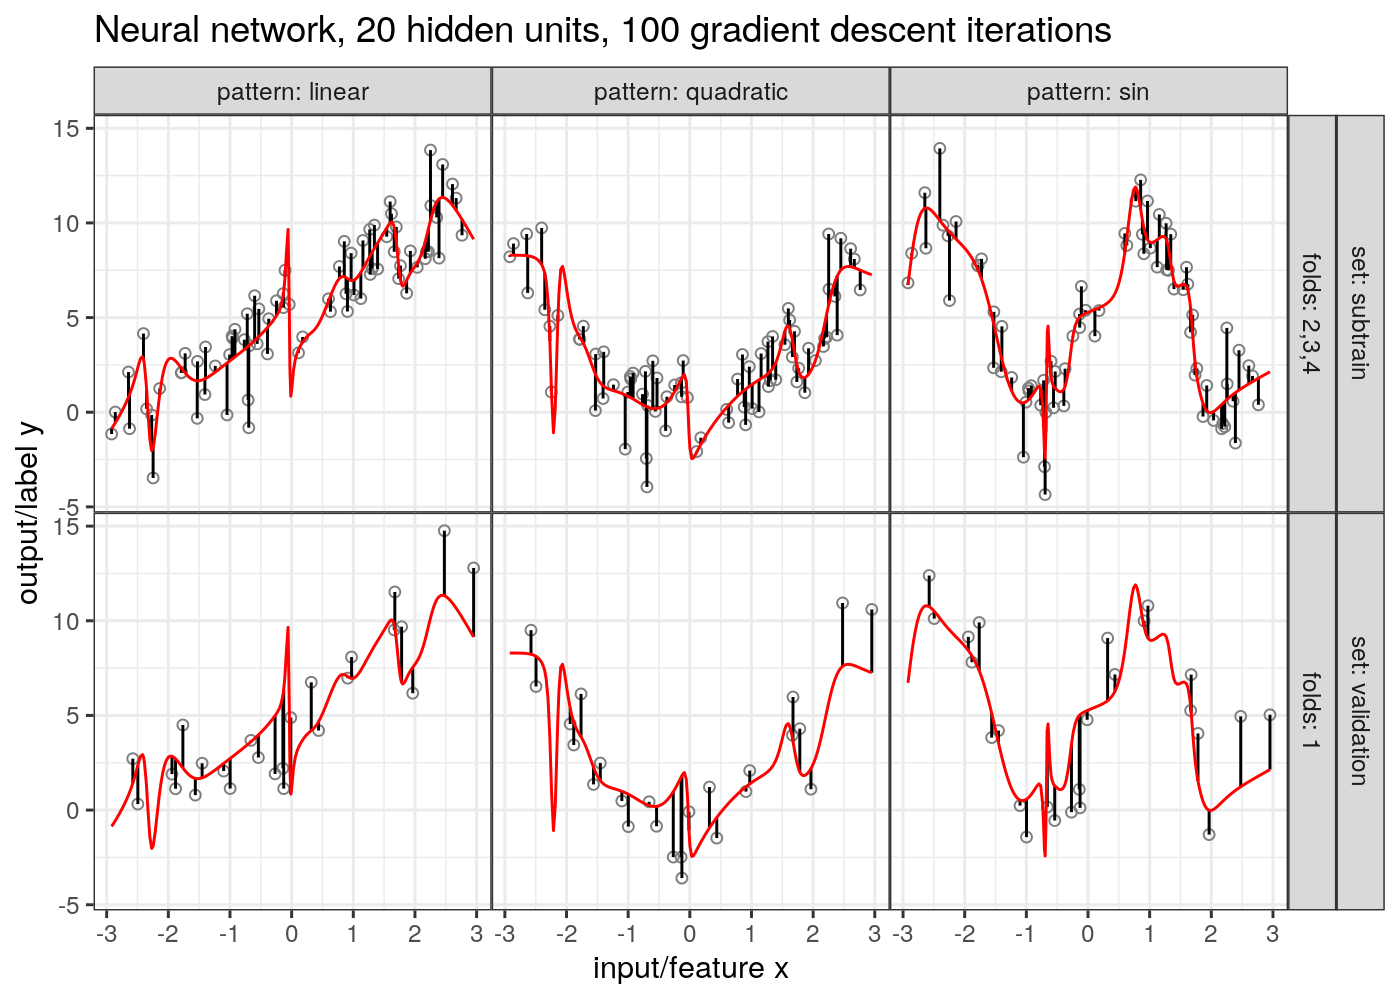
\includegraphics[width=\textwidth]{figure-overfitting-pred-units=20-maxit=100.png}
\
Data=grey dots, predictions=red curve, loss=black vertical line segments.
\end{frame}


\begin{frame}
  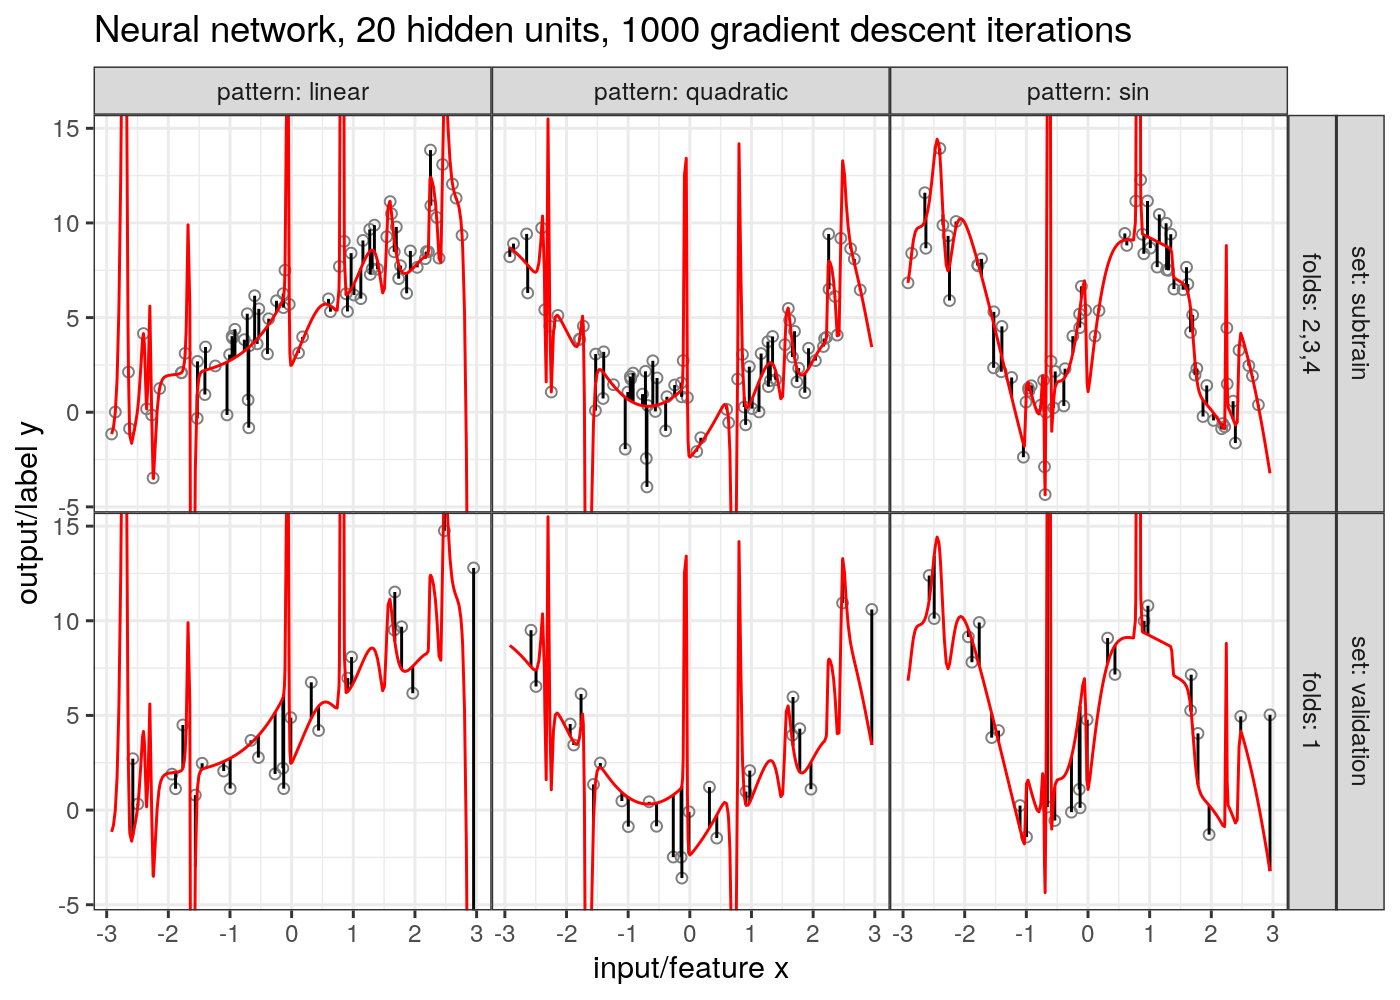
\includegraphics[width=\textwidth]{figure-overfitting-pred-units=20-maxit=1000.png}
\
Data=grey dots, predictions=red curve, loss=black vertical line segments.
\end{frame}


\begin{frame}
  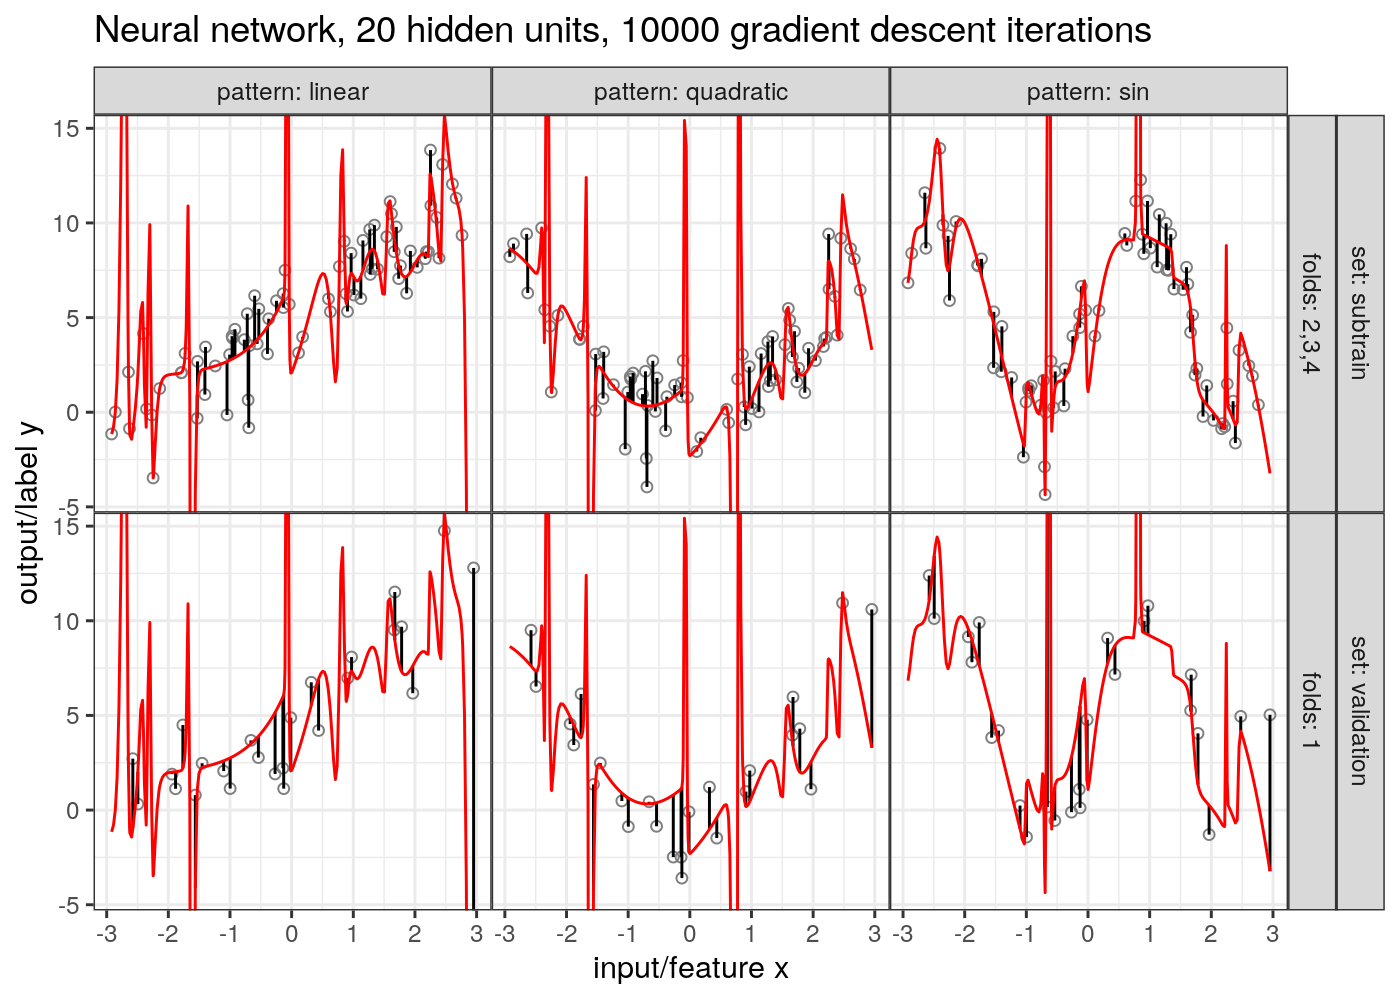
\includegraphics[width=\textwidth]{figure-overfitting-pred-units=20-maxit=10000.png}
\
Data=grey dots, predictions=red curve, loss=black vertical line segments.
\end{frame}


\begin{frame}
  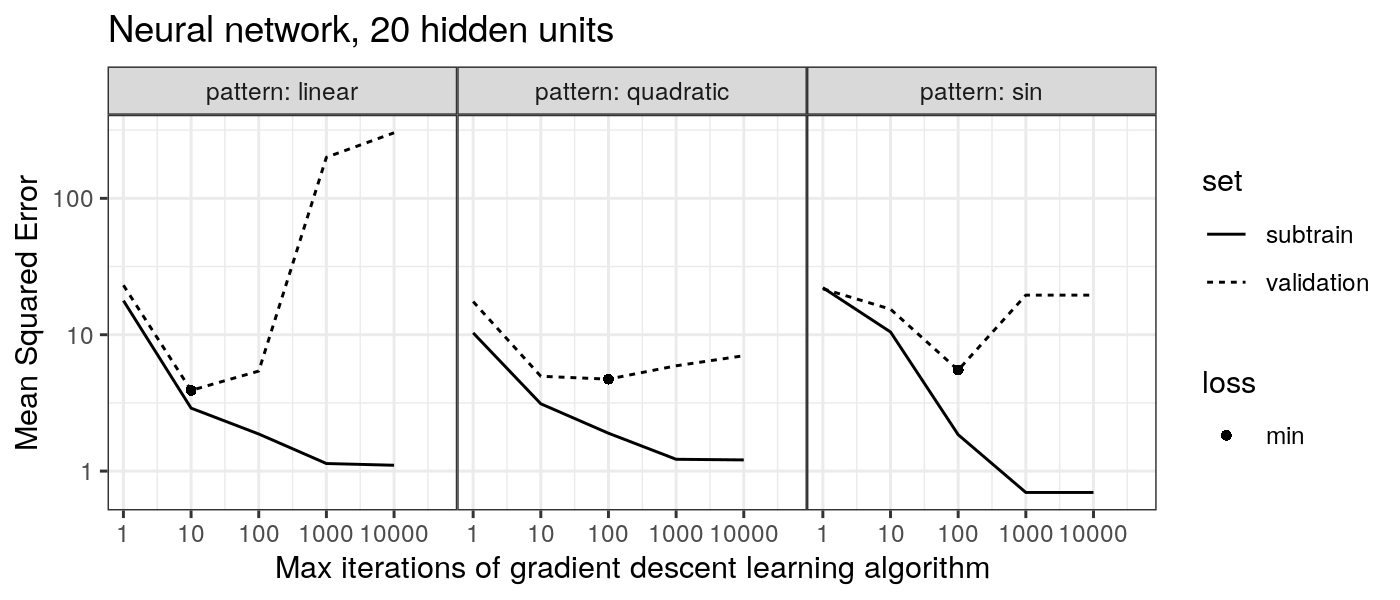
\includegraphics[width=\textwidth]{figure-overfitting-data-loss-20.png}
\
Data=grey dots, predictions=red curve, loss=black vertical line segments.
\end{frame}

 

\begin{frame}
  \frametitle{Neural network prediction function} For an input feature
  vector $\mathbf x\in\mathbb R^{u_1}$, the prediction function for a
  neural network with $L$ layers (functions to learn) is:
\begin{equation}
  f(\mathbf x) = f_L[\cdots f_1[\mathbf x] ].
\end{equation}
  We have for all $l\in\{1,\dots,L\}$:
\begin{equation}
  f_l(t) = A_l( \mathbf W_l^\intercal t ),
\end{equation}
The hyper-parameters which must be fixed prior to learning:
\begin{itemize}
\item Number of functions to learn $L$.
\item Activation functions $A_l$ (classically sigmoid, typically ReLU).
\item Number of hidden units per layer ($u_1,\dots,u_{L-1}$).
\item Sparsity pattern in the weight matrices $\mathbf W_l\in\mathbb R^{u_{l}\times u_{l-1}}$.
\end{itemize}
\end{frame}

\begin{frame}
  \frametitle{Network for 1 input, 1 output, 1 hidden layer}
  Neural network
  diagrams show how each unit (node) is computed by applying the
  weights (edges) to the values of the units at the previous layer.

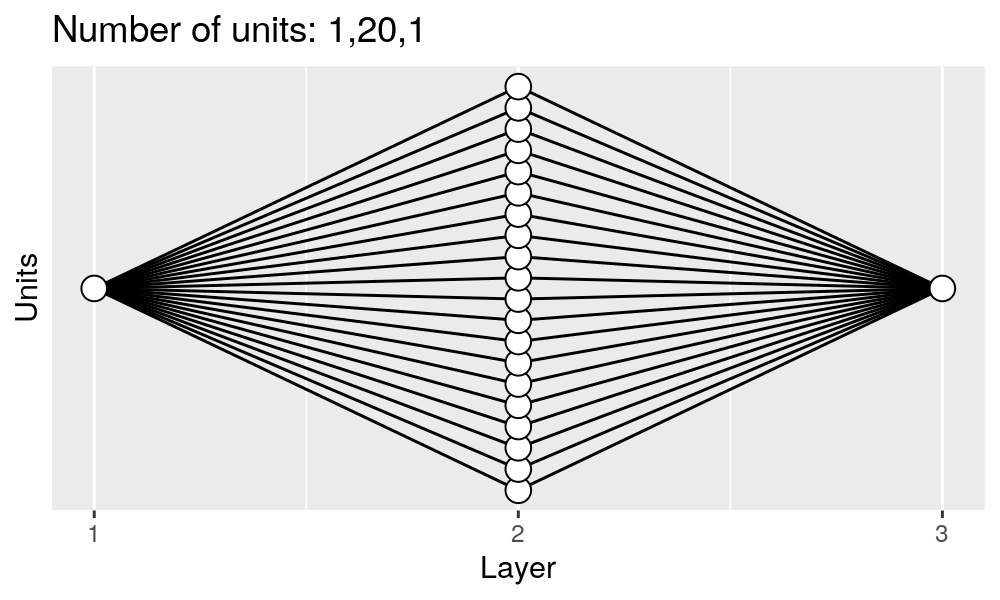
\includegraphics[width=\textwidth]{figure-architecture-reg20}
\end{frame}

\begin{frame}
  \frametitle{Network for 12 inputs, 1 output, 1 hidden layer}
  Neural network
  diagrams show how each unit (node) is computed by applying the
  weights (edges) to the values of the units at the previous layer.

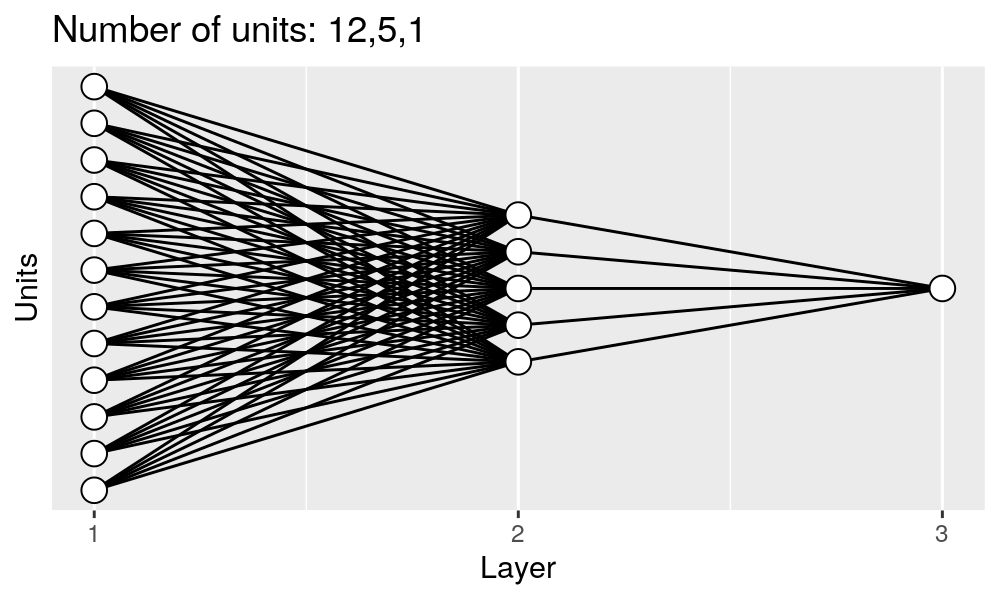
\includegraphics[width=\textwidth]{figure-architecture-oneOut}
\end{frame}

\begin{frame}
  \frametitle{Network for 12 inputs, 10 outputs, 1 hidden layer}
  Neural network
  diagrams show how each unit (node) is computed by applying the
  weights (edges) to the values of the units at the previous layer.

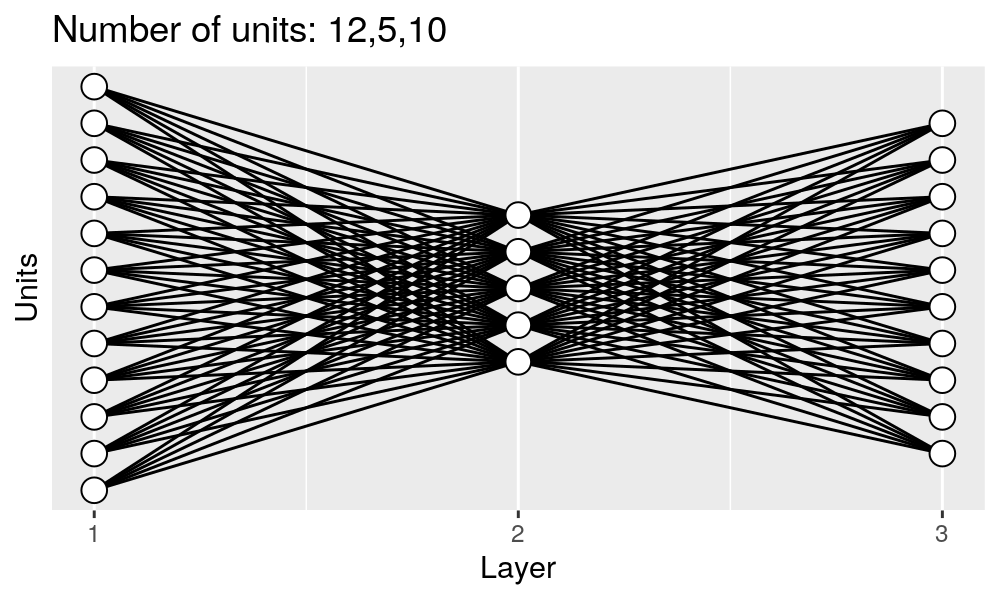
\includegraphics[width=\textwidth]{figure-architecture-tenOut}
\end{frame}

\begin{frame}
  \frametitle{Network for 4 inputs, 1 output, 3 hidden layers}
  Neural network
  diagrams show how each unit (node) is computed by applying the
  weights (edges) to the values of the units at the previous layer.

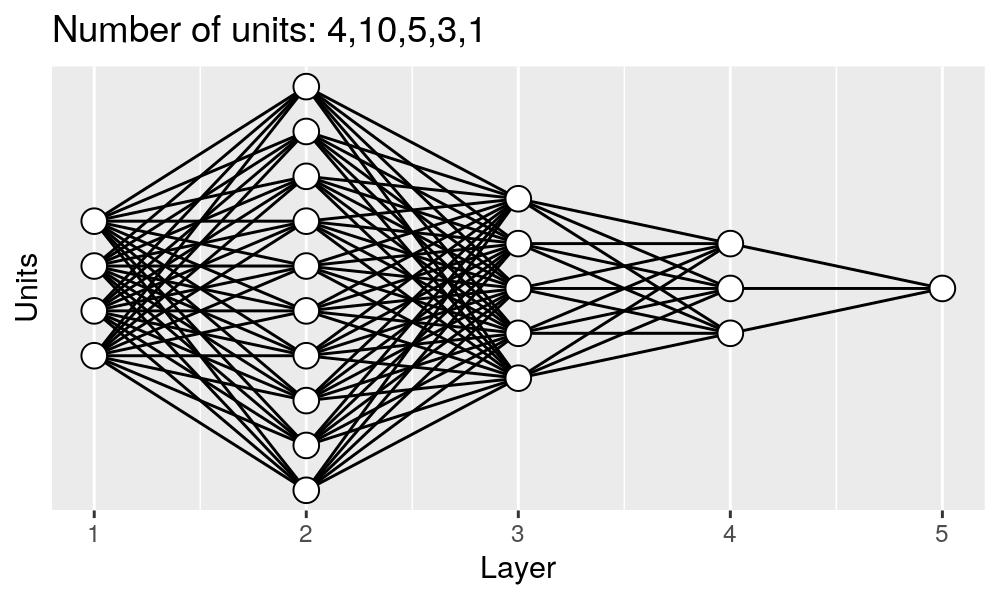
\includegraphics[width=\textwidth]{figure-architecture-fiveLayers}
\end{frame}


\begin{frame}
  \frametitle{Non-linear activation functions $A_l$}
  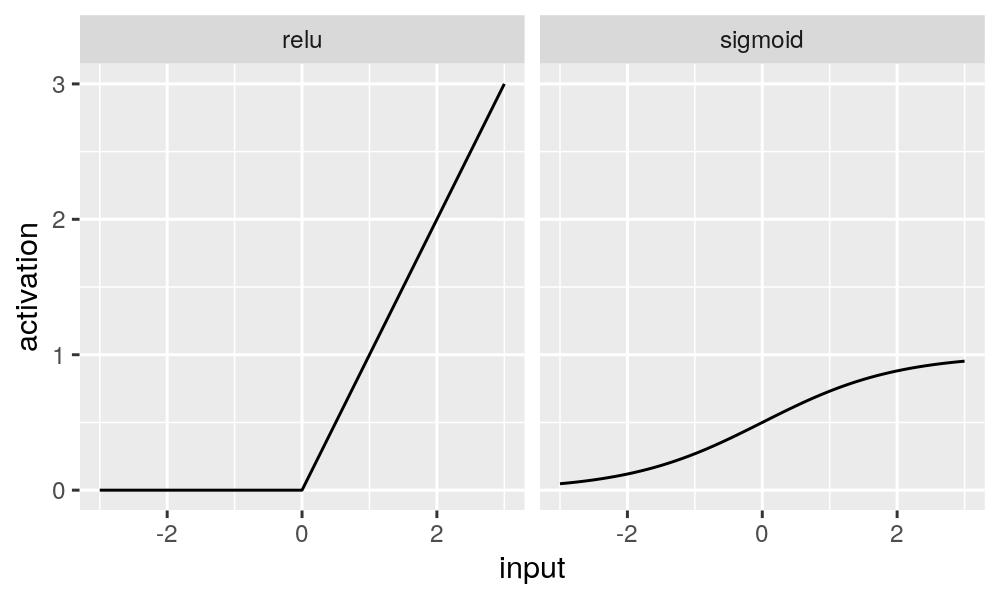
\includegraphics[width=\textwidth]{figure-activations}

Each layer except the last should have a activation function $A_l$
which is not linear (last layer activation should be identity/linear).
\end{frame}

\begin{frame}
  \frametitle{Gradient Descent Learning}

  The neural network prediction function
  $f(\mathbf x) = f_L[\cdots f_1[\mathbf x] ]$ has $l\in\{1,\dots,L\}$
  component functions to learn:
\begin{equation}
  f_l(t) = A_l( \mathbf W_l^\intercal t ),
\end{equation}
The weight matrices $\mathbf W_l\in\mathbb R^{u_l\times u_{l-1}}$ are
learned using gradient descent.
\begin{itemize}
\item A loss function $\mathcal L[f(\mathbf x), y]$ computes how bad
  are predictions with respect to labels $y$ (ex: mean squared error
  for regression, cross entropy loss for classification).
\item In each \textbf{iteration} of gradient descent, the weights are
  updated in order to get better predictions on subtrain data.
\item An \textbf{epoch} computes gradients on all subtrain data;
  there can be from 1 to $N$(subtrain size) iterations per epoch.
\end{itemize}
\end{frame}


\begin{frame}
  \centering
  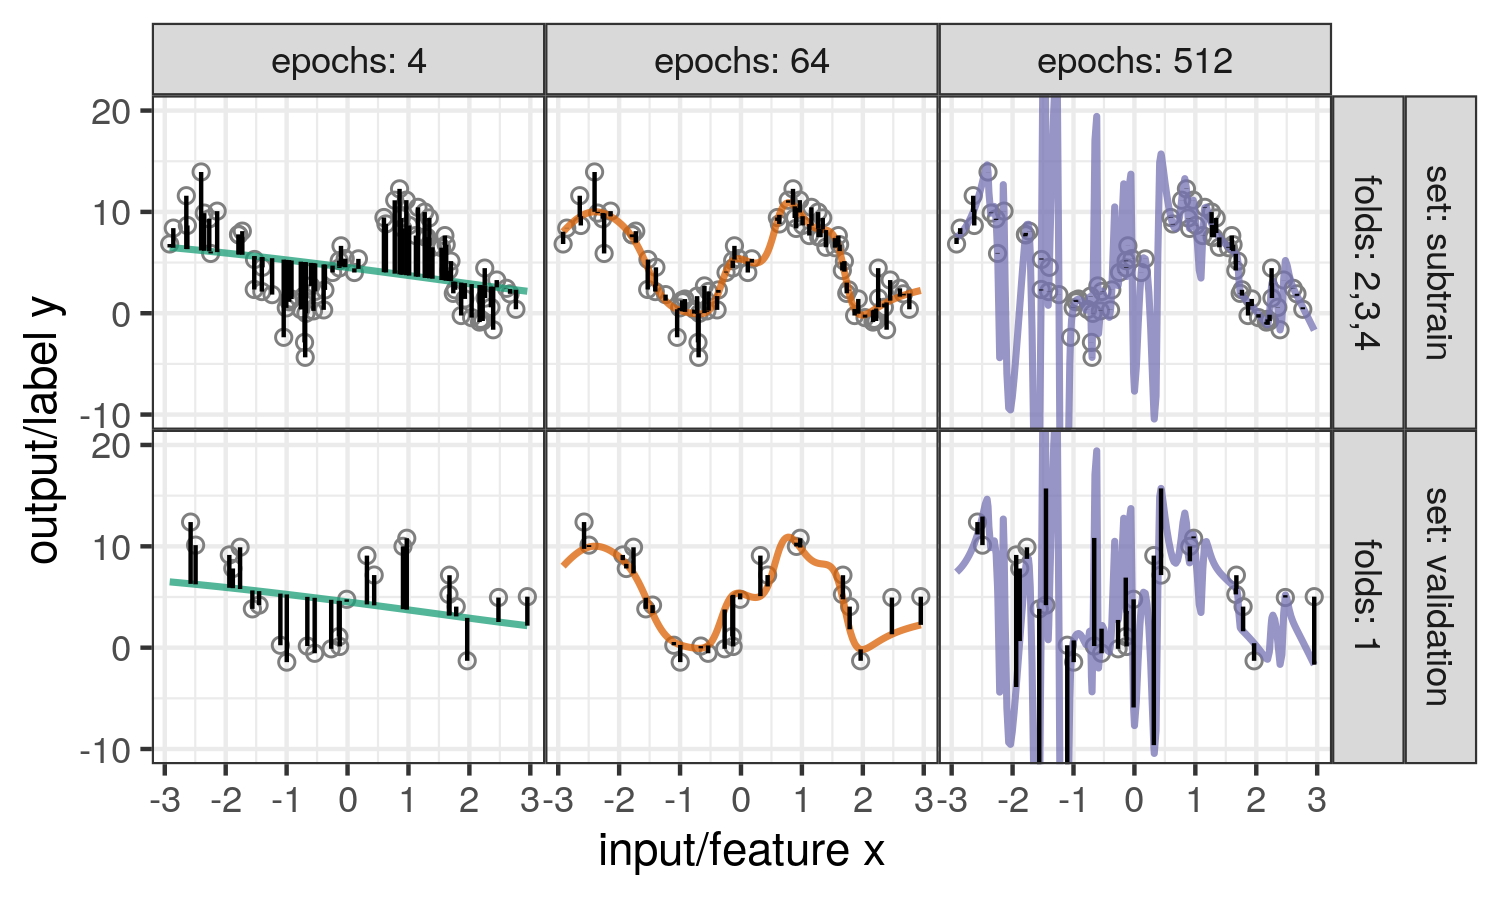
\includegraphics[height=0.5\textheight]{figure-overfitting-paper}
  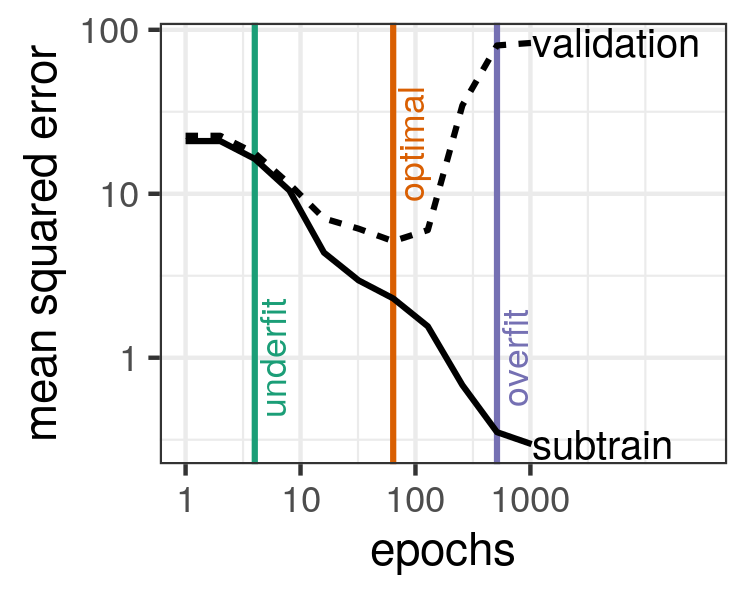
\includegraphics[height=0.45\textheight]{figure-overfitting-paper-loss}   
\end{frame} 

\begin{frame}
  \frametitle{Summary of how to avoid overfitting}
  \begin{itemize}
  \item Happens when subtrain error/loss decreases but validation error
    increases (as a function of some hyper-parameter)
  \item Here the hyper-parameter is the number of iterations of
    gradient descent, and overfitting starts after a certain number of
    iterations.
  \item To maximize prediction accuracy you need to choose a
    hyper-parameter with minimal validation error/loss.
  \item This optimal hyper-parameter will depend on the data set.
  \item To get optimal prediction accuracy in any machine learning
    analysis, you always need to do this, because you never know the
    best hyper-parameters in advance.
  \end{itemize}
\end{frame}

\section{Example 2: classifying images of digits, coding demos  
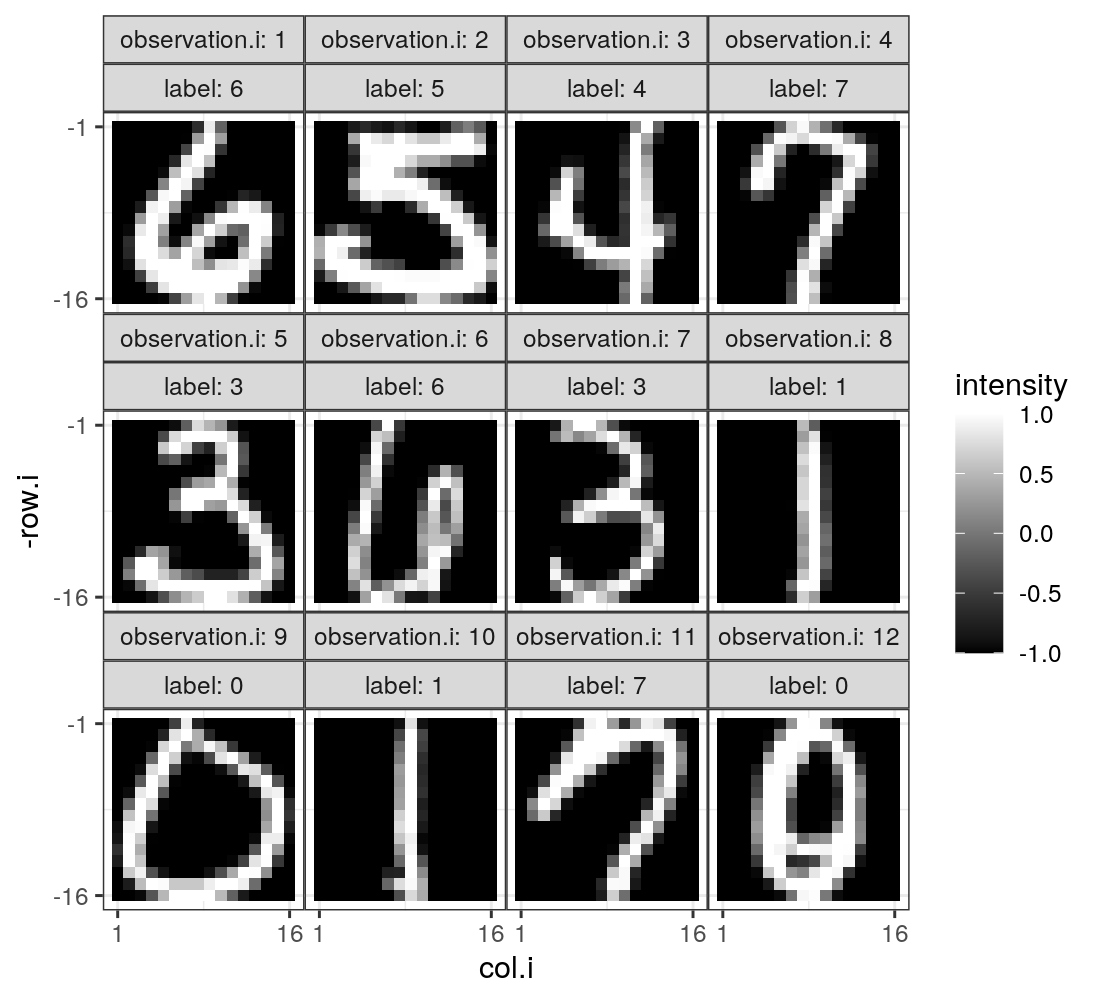
\includegraphics[height=3cm]{figure-validation-loss-digits}}

\begin{frame}
  \frametitle{Image classification}
  \begin{itemize}
  \item A problem in computer vision, one of the most
    popular/successful application domains of machine learning.
  \item Input: image file $x\in\mathbb R^{h\times w\times c}$ where
    $h$ is the height in pixels, $w$ is the width, $c$ is the number
    of channels, e.g. RGB image $c=3$ channels.
  \item In this tutorial we use images with $h=w=16$ pixels and $c=1$
    channel (grayscale, smaller values are darker).
  \item Output: class/category $y$ (from a finite set).
  \item In this tutorial there are ten image classes $y\in\{0, 1, \dots, 9\}$, one for each
    digit.
  \item Want to learn $f$ such that
    $f(
\includegraphics[height=1cm]{mnist-0})=0$,
    $f(
\includegraphics[height=1cm]{mnist-1})=1$, etc.
  \item Code for figures in this section:
    \url{https://github.com/tdhock/2023-res-baz-az/blob/main/figure-validation-loss.R}
  \end{itemize}
\end{frame}

\begin{frame}
  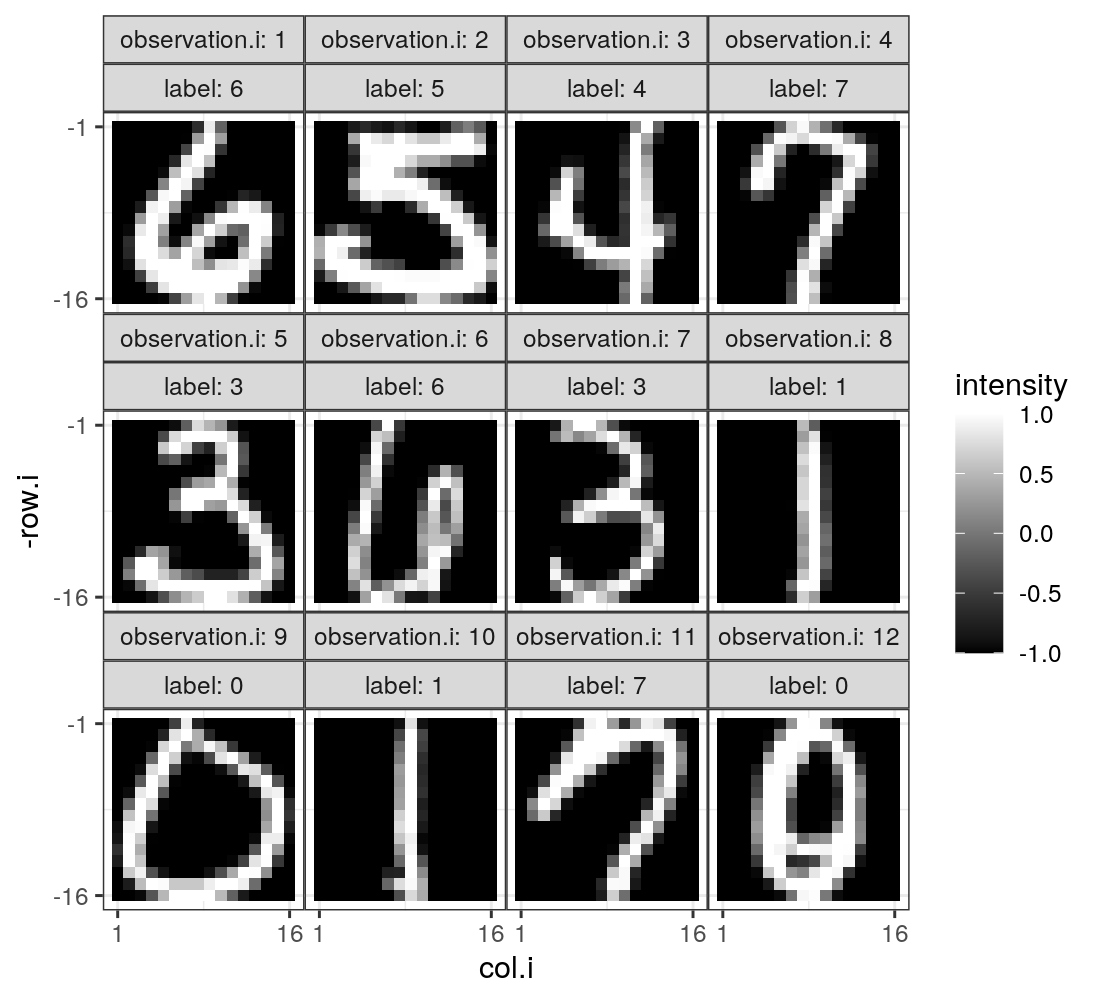
\includegraphics[height=\textheight]{figure-validation-loss-digits}
\end{frame}

\begin{frame}[fragile]
  \frametitle{Representation of digits in CSV}

  \begin{itemize}
  \item Each image/observation is one row.
  \item First column is output/label/class to predict.
  \item Other 256 columns are inputs/features (pixel intensity
    values).
  \end{itemize}
 Data from {\scriptsize \url{https://web.stanford.edu/~hastie/ElemStatLearn/datasets/zip.train.gz}}

\begin{verbatim}
 1:  6 -1 -1  ... -1.000 -1.000   -1
 2:  5 -1 -1  ... -0.671 -0.828   -1
 3:  4 -1 -1  ... -1.000 -1.000   -1
 4:  7 -1 -1  ... -1.000 -1.000   -1
 5:  3 -1 -1  ... -0.883 -1.000   -1
 6:  6 -1 -1  ... -1.000 -1.000   -1
...
\end{verbatim}

Demo: reading CSV, plotting digits, \url{https://github.com/tdhock/2023-res-baz-az/blob/main/2023-04-19-deep-learning.Rmd}
  
\end{frame}

\begin{frame}[fragile]
  \frametitle{Converting R data to torch tensors}
Use array function with all columns except first as data.  
\begin{verbatim}
zip.dt <- data.table::fread("zip.train.gz")
zip.X.array <- array(
  data = unlist(zip.dt[,-1]),
  dim = c(nrow(zip.dt), 1, 16, 16))
zip.X.tensor <- torch::torch_tensor(zip.X.array)
zip.y.tensor <- torch::torch_tensor(
  zip.dt$V1+1L, torch::torch_long())
\end{verbatim}
Need to specify dimensions of input/X array:
\begin{itemize}
\item Observations: same as the number of rows in the CSV table.
\item Channels: 1 (greyscale image, would be 3 for RGB image).
\item Pixels wide: 16.
\item Pixels high: 16.
\end{itemize}

For output/y need to add 1 in R, and specify long int type.

\end{frame}

\begin{frame}[fragile]
  \frametitle{Linear model R code}

\begin{verbatim}
n.features <- 16*16
n.classes <- 10
linear.model <- torch::nn_sequential(
  torch::nn_flatten(),
  torch::nn_linear(n.features, n.classes))
pred.tensor <- linear.model(zip.X.tensor)
\end{verbatim}

  \begin{itemize}
  \item First layer must specify shape of inputs (here 16x16x1).
  \item \texttt{nn\_flatten} converts any shape to a single dimension
    of units (here, convert each image from 1x16x16-array to 256-vector).
  \item \texttt{nn\_linear} uses all units/features in the previous
    layer (256) to predict each unit in the next layer (10).
  \item There are ten possible classes for an output.
  \end{itemize}

\end{frame}

\begin{frame}[fragile]
\frametitle{Loss computation}
\begin{verbatim}
loss.fun <- torch::nn_cross_entropy_loss()
loss.tensor <- loss.fun(pred.tensor, zip.y.tensor)
step.size <- 0.1
optimizer <- torch::optim_sgd(
  linear.model$parameters, lr=step.size)
optimizer$zero_grad()
loss.tensor$backward()
optimizer$step()
\end{verbatim}
\begin{itemize}
\item \texttt{loss.fun} is the cross-entropy loss for multi-class
  classification, which is directly optimized/minimized in each
  iteration of the gradient descent learning algorithm.
\item \texttt{optimizer} is the version of the gradient descent learning
  algorithm to use.
\item \texttt{backward} method computes gradients.
\item \texttt{step} method updates model parameters based on gradients.
\end{itemize}
\end{frame}

\begin{frame}[fragile]
  \frametitle{Gradient Descent learning algorithm}
\begin{verbatim}
gradient_descent <- 
  function(index.list, model, n_epochs, gradient.set){
  loss.dt.list <- list()
  for(epoch in seq(1, n_epochs)){
    take_steps(index.list[[gradient.set]], model)
    epoch.loss.dt <- loss_each_set(index.list, model)
    loss.dt.list[[paste(epoch)]] <- 
      data.table(epoch, epoch.loss.dt)
  }
  rbindlist(loss.dt.list)
}
\end{verbatim}
  \begin{itemize}
  \item \verb|take_steps| sub-routine updates model parameters.
  \item \verb|loss_each_set| computes loss and error rate on gradient set
    and held-out set.
  \end{itemize}
\end{frame}
 
\begin{frame}
  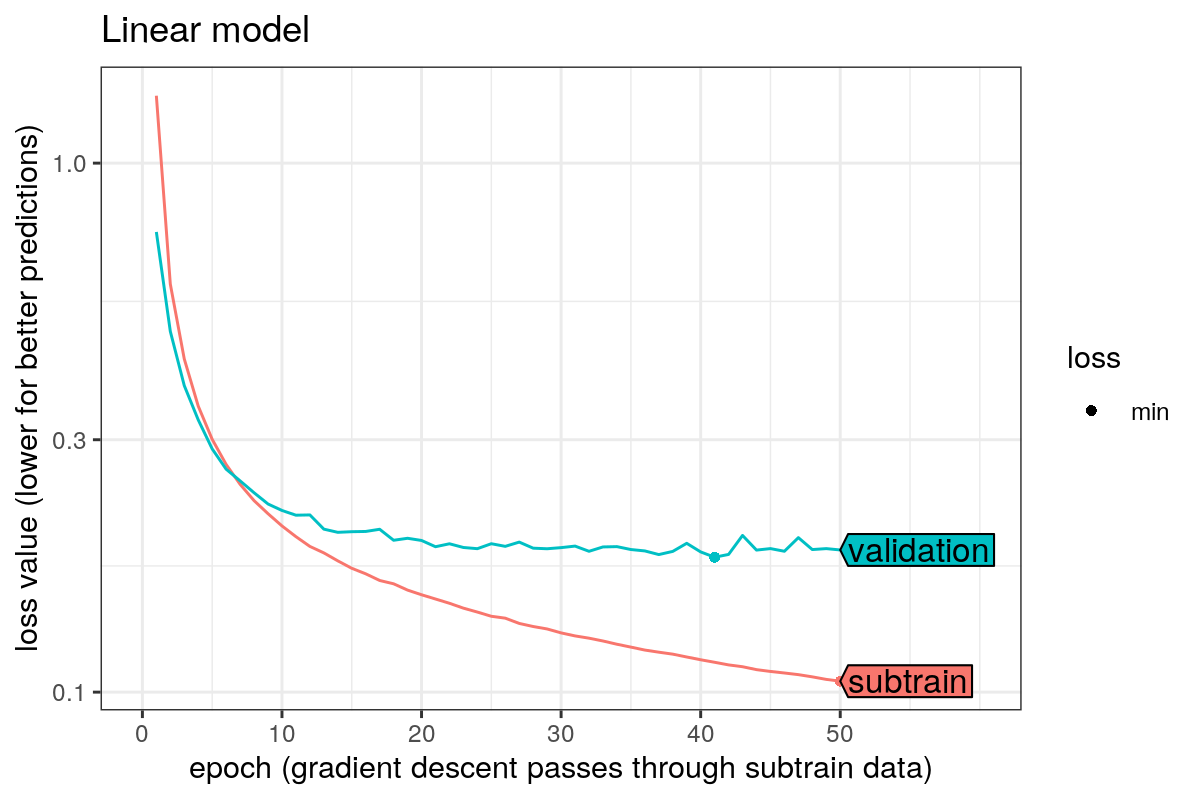
\includegraphics[width=\textwidth]{figure-validation-loss-linear}

  Demo: splitting data, gradient descent loop.
\end{frame}
 
\begin{frame}[fragile]
  \frametitle{Dense (fully connected) neural network R code}

\begin{verbatim}
one.hidden.layer <- torch::nn_sequential(
  torch::nn_flatten(),
    torch::nn_linear(n.features, n.hidden.units),
    torch::nn_relu(),
    torch::nn_linear(n.hidden.units, n.classes))
two.hidden.layers <- torch::nn_sequential(
  torch::nn_flatten(),
    torch::nn_linear(n.features, n.hidden.1),
    torch::nn_relu(),
    torch::nn_linear(n.hidden.1, n.hidden.2),
    torch::nn_relu(),
    torch::nn_linear(n.hidden.2, n.classes))
\end{verbatim}

\end{frame}

\begin{frame}[fragile]
  \frametitle{Use for loop to implement dense network}
\begin{verbatim}
new_fully_connected_units <- function(units.per.layer){
  seq.args <- list(torch::nn_flatten())
  for(output.i in seq(2, length(units.per.layer))){
    input.i <- output.i-1
    seq.args[[length(seq.args)+1]] <- torch::nn_linear(
      units.per.layer[[input.i]], 
      units.per.layer[[output.i]])
    if(output.i<length(units.per.layer)){
      seq.args[[length(seq.args)+1]] <- torch::nn_relu()
    }
  }
  do.call(torch::nn_sequential, seq.args)
}
\end{verbatim}
  \begin{itemize}
  \item input a vector of units per layer, for example c(256,1000,100,10).
  \item Begin with flatten.
  \item Linear followed by relu in each layer except last.
  \end{itemize}
\end{frame}
 
\begin{frame}
  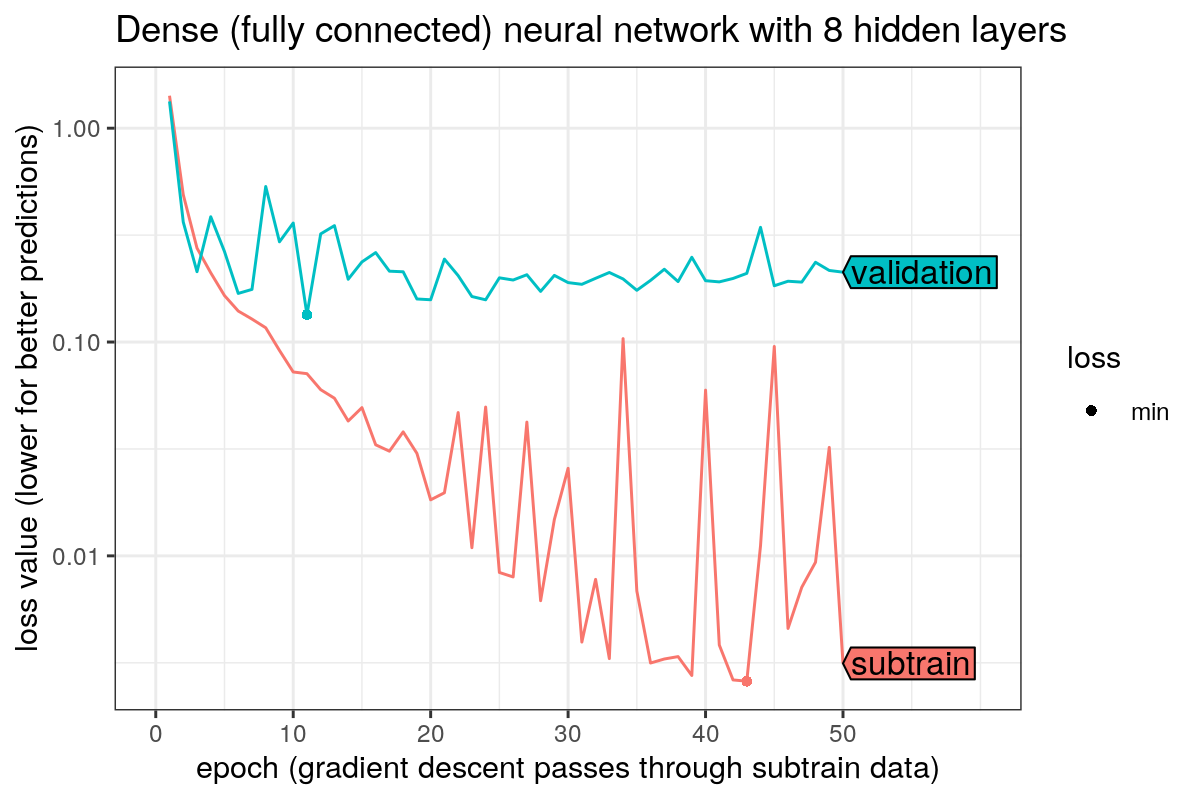
\includegraphics[width=\textwidth]{figure-validation-loss-dense}
\end{frame}
 
\begin{frame}
  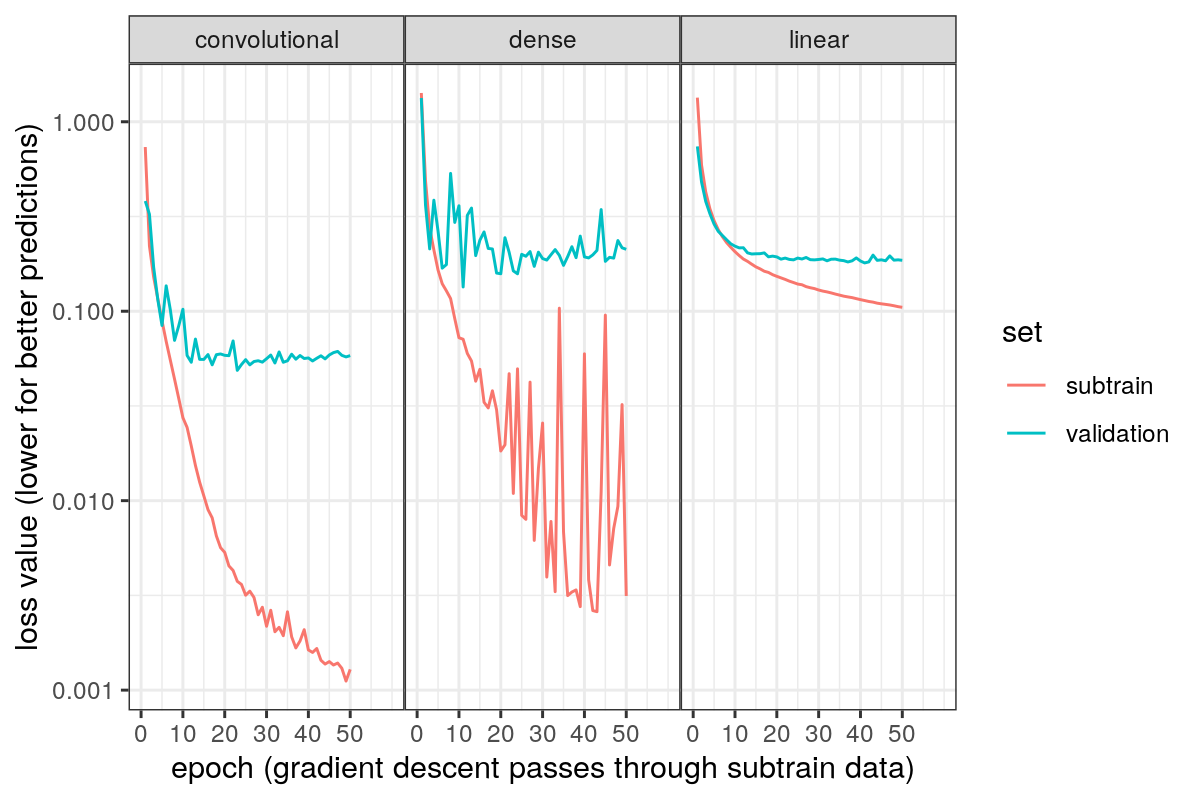
\includegraphics[width=\textwidth]{figure-validation-loss-three}
\end{frame}

\begin{frame}[fragile]
  \frametitle{Fully connected/dense vs convolutional/sparse network}
  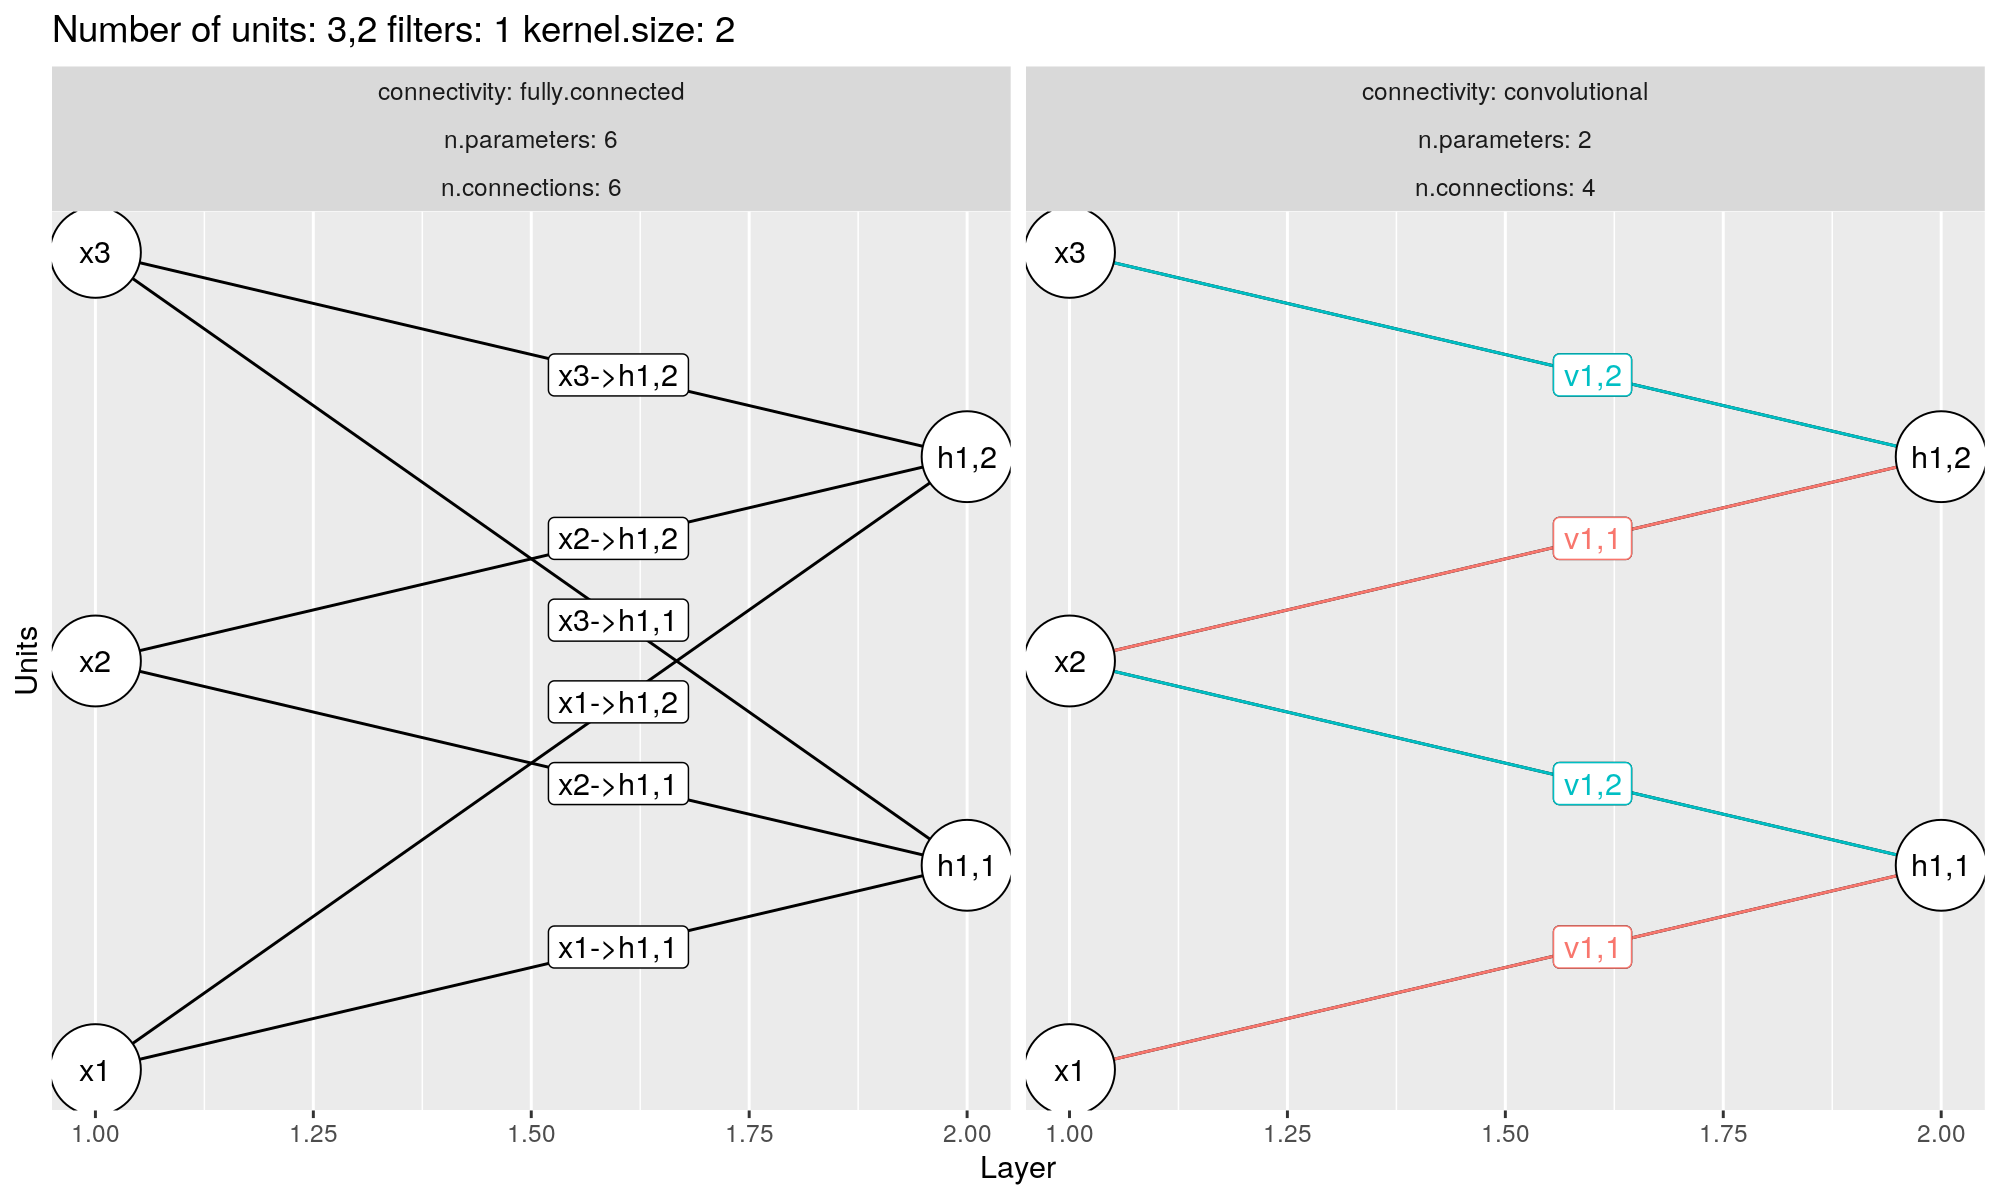
\includegraphics[width=\textwidth]{figure-convolutional-filters-3-2-1}
\begin{verbatim}
torch::nn_conv1d(in_channels=1, 
  out_channels=1, kernel_size=2)
\end{verbatim}

\end{frame}

\begin{frame}[fragile]
  \frametitle{Convolutional with two filters/output channels}
  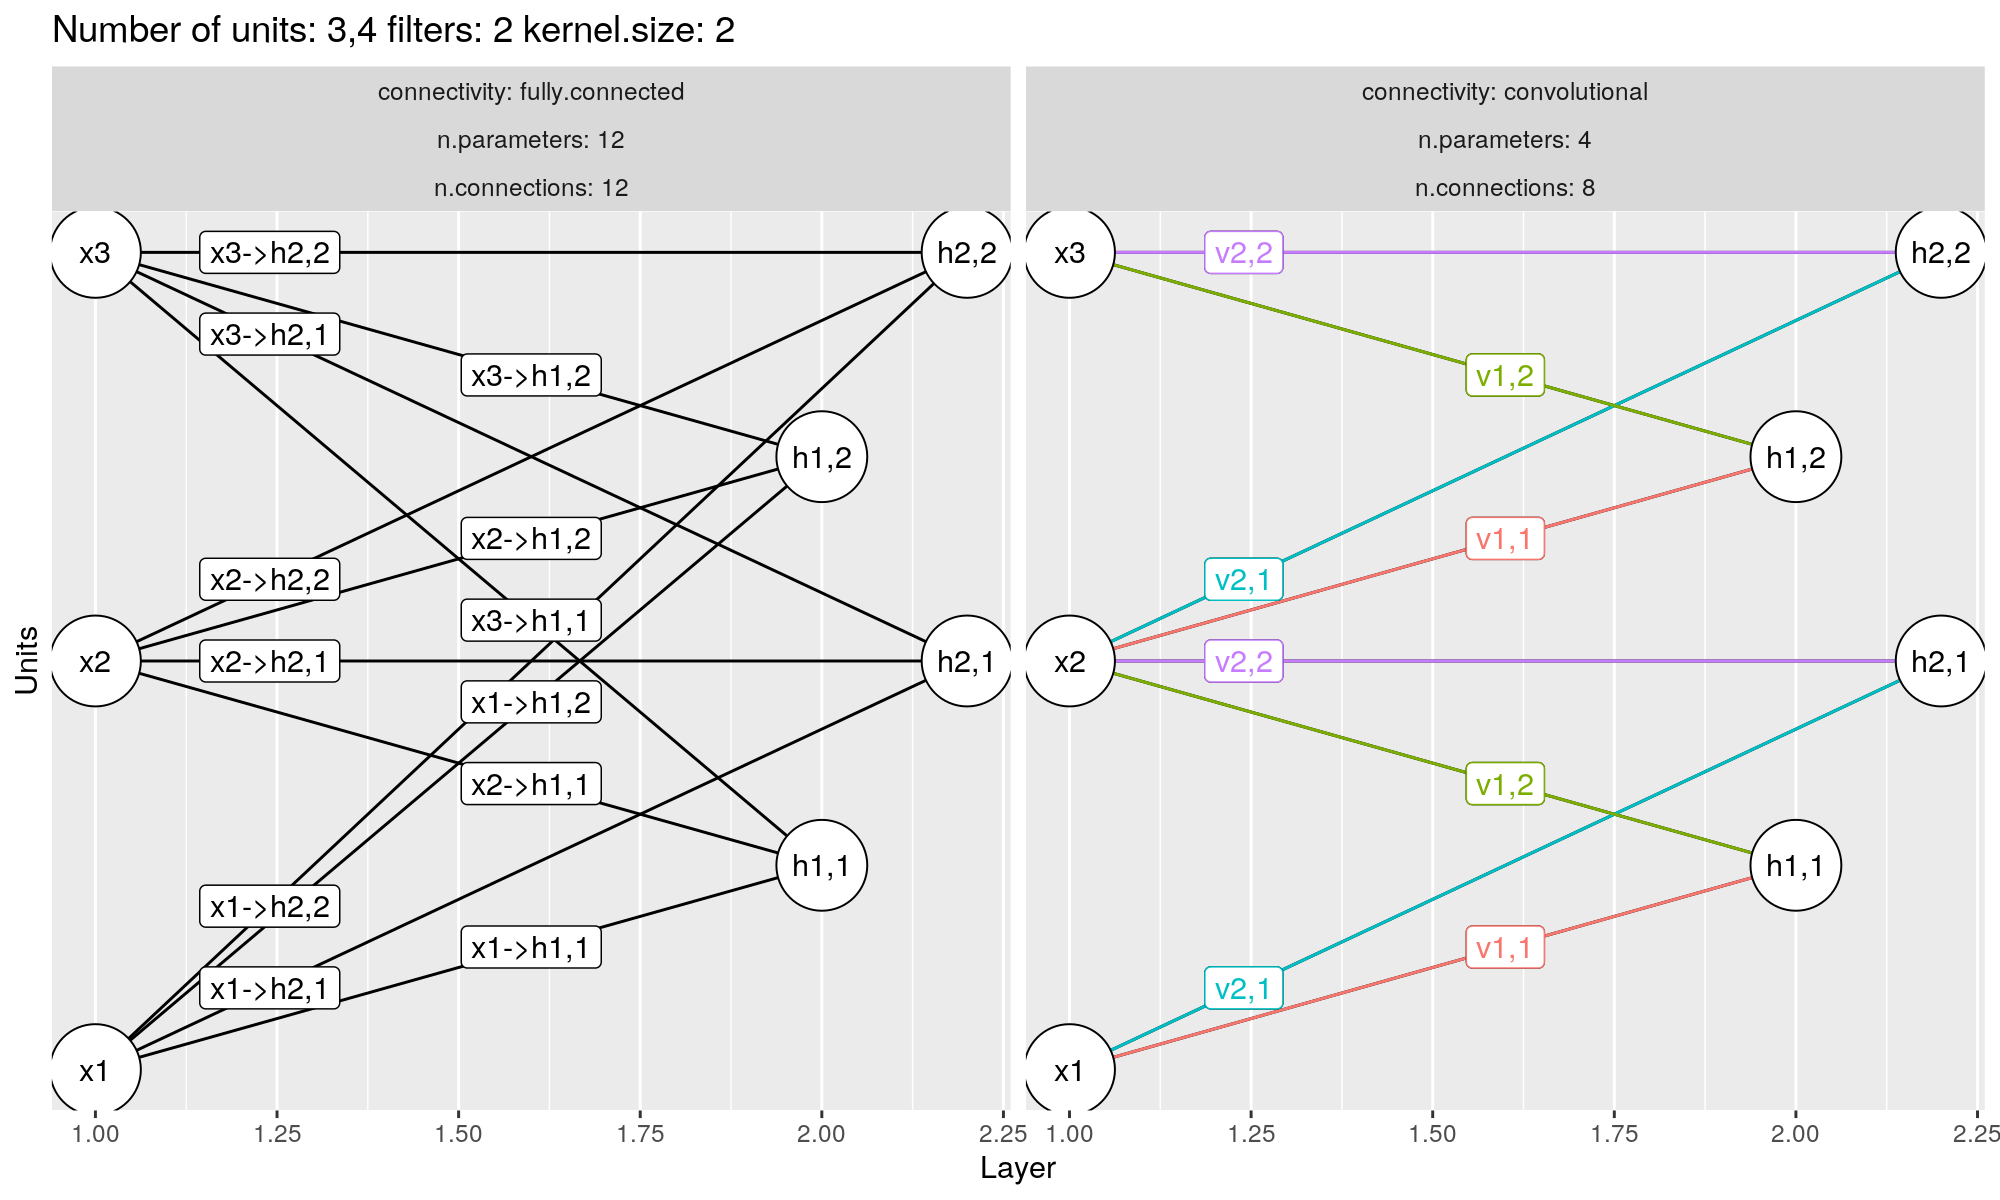
\includegraphics[width=\textwidth]{figure-convolutional-filters-3-2-2}
  
\begin{verbatim}
torch::nn_conv1d(in_channels=1, 
  out_channels=2, kernel_size=2)
\end{verbatim}
\end{frame}

\begin{frame}[fragile]
  \frametitle{Fully connected vs convolutional, two filters}
  \begin{eqnarray*}
  \begin{bmatrix}
    h_1 \\
    h_2 
  \end{bmatrix}
    &=&
  \begin{bmatrix}
    w_{1,1} & w_{1,2} & w_{1,3} \\
    w_{2,1} & w_{2,2} & w_{2,3}
  \end{bmatrix}
  \begin{bmatrix}
    x_1 \\
    x_2 \\
    x_3
  \end{bmatrix} \text{(fully connected)}
    \\
  \begin{bmatrix}
    h_1 \\
    h_2 
  \end{bmatrix}
    &=&
  \begin{bmatrix}
    v_{1} & v_{2} & 0 \\
    0 & v_{1} & v_{2}
  \end{bmatrix}
  \begin{bmatrix}
    x_1 \\
    x_2 \\
    x_3
  \end{bmatrix} \text{(convolutional)}\\
  \begin{bmatrix}
    h_{1,1} \\
    h_{1,2} \\
    h_{2,1} \\
    h_{2,2}
  \end{bmatrix}
    &=&
  \begin{bmatrix}
    v_{1,1} & v_{1,2} & 0 \\
    0 & v_{1,1} & v_{1,2} \\
    v_{2,1} & v_{2,2} & 0 \\
    0 & v_{2,1} & v_{2,2}
  \end{bmatrix}
  \begin{bmatrix}
    x_1 \\
    x_2 \\
    x_3
  \end{bmatrix} \text{(conv, two filters)}
  \end{eqnarray*}
  \begin{itemize}
  \item Weight sharing: same weights used to compute different
    output units. 
  \item Sparsity: zeros in weight matrix.
  \end{itemize}
\end{frame}

\begin{frame}[fragile]
  \frametitle{Sparse (convolutional) model R code}

\begin{verbatim}
seq2flat <- torch::nn_sequential(
  torch::nn_conv2d(in_channels = 1, out_channels = 10, kernel_size = 4),
  torch::nn_relu(),
  torch::nn_max_pool2d(kernel_size = 2),
  torch::nn_flatten())
one.flat <- seq2flat(zip.X.tensor[1,,,,drop=FALSE])
n.flat <- length(one.flat)
torch::nn_sequential(
  seq2flat, 
  torch::nn_linear(n.flat, n.hidden.units),
  torch::nn_relu(),
  torch::nn_linear(n.hidden.units, n.classes))
\end{verbatim}

  \begin{itemize}
  \item Sparse: few inputs are used to predict each unit in
    \texttt{nn\_conv2d}.
  \item Exploits structure of image data to make learning
    easier/faster.
  \end{itemize}

\end{frame}
 
\begin{frame}
  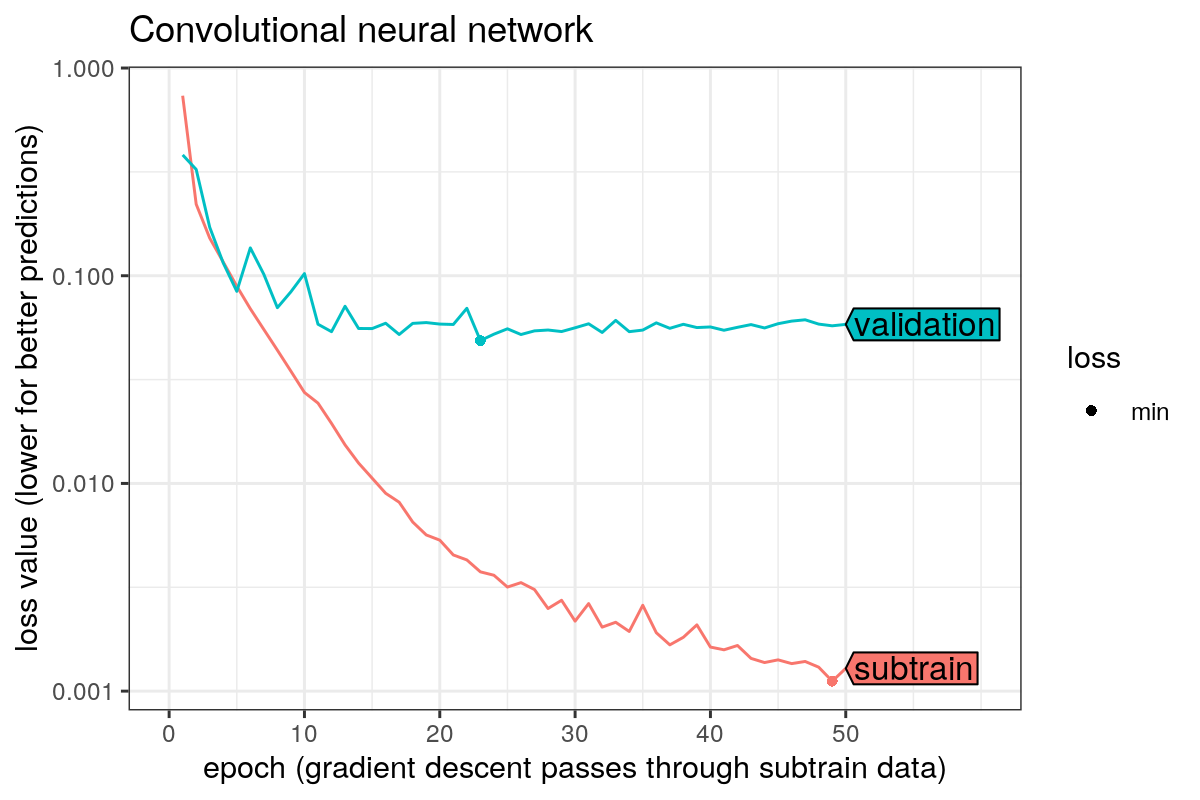
\includegraphics[width=\textwidth]{figure-validation-loss-conv}
\end{frame}
 
\begin{frame}
  \frametitle{K-fold cross-validation for model evaluation}
  Is convolutional more accurate on unseen test data?
  
  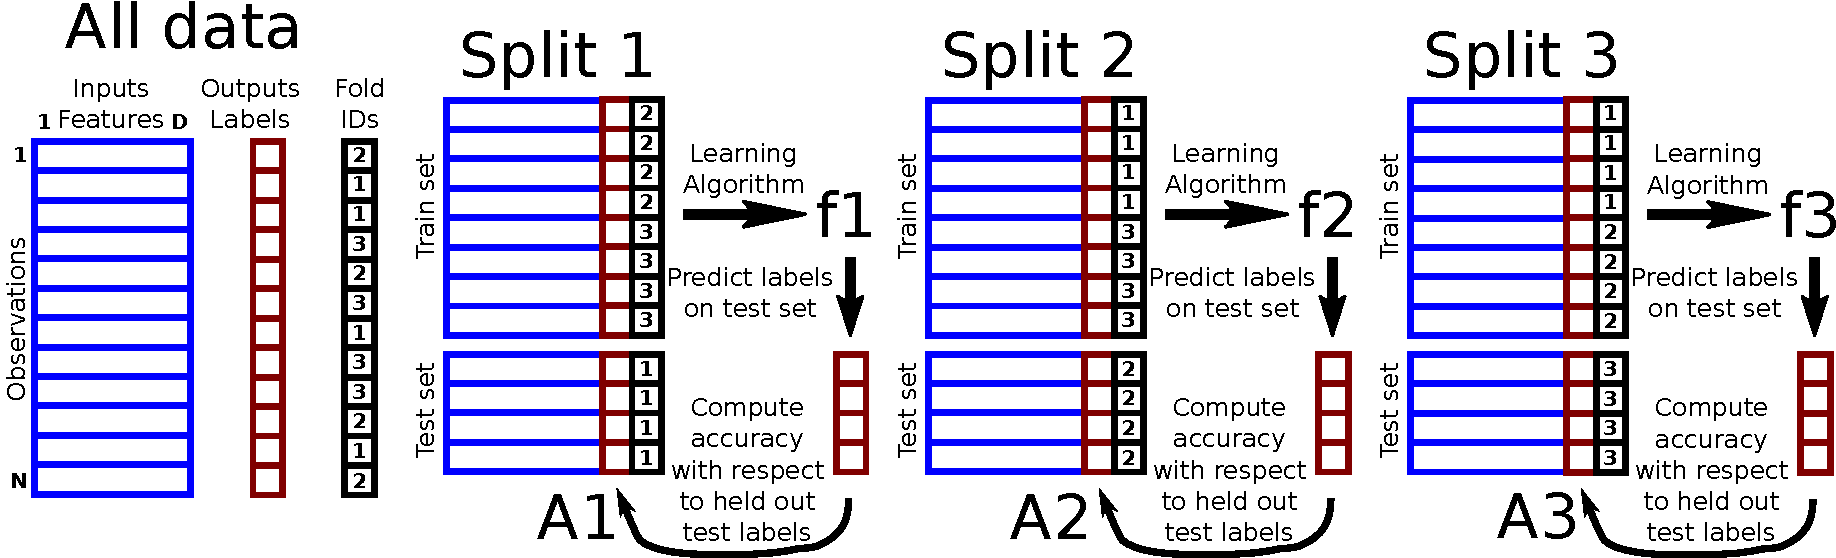
\includegraphics[width=\textwidth]{drawing-cross-validation}
  
  \begin{itemize}
  \item Randomly assign a fold ID from 1 to K to each observation.
  \item Hold out the observations with the Split ID as test set.
  \item Use the other observations as the train set.
  \item Run learning algorithm on train set (including hyper-parmeter
    selection), outputs learned function (f1-f3).
  \item Finally compute and plot the prediction accuracy (A1-A3) with
    respect to the held-out test set.
  \end{itemize}
\end{frame}


 

\begin{frame}
  \frametitle{Two kinds of cross-validation must be used}
  
  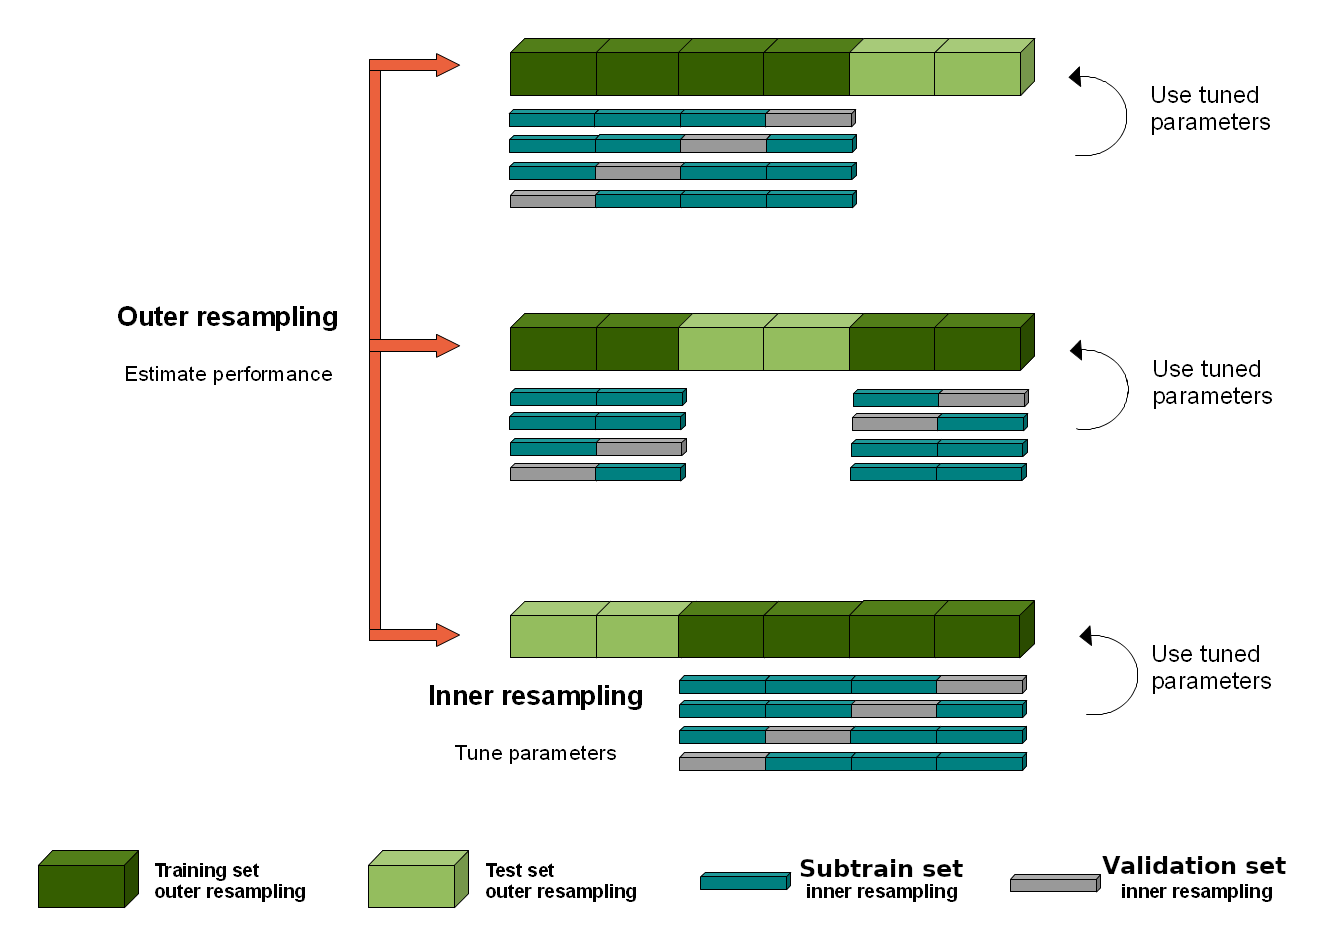
\includegraphics[width=\textwidth]{nested_resampling.png}

  Source: \url{https://mlr.mlr-org.com/articles/tutorial/nested_resampling.html}
\end{frame}


\begin{frame}
  \frametitle{Accuracy rates for each test fold}
  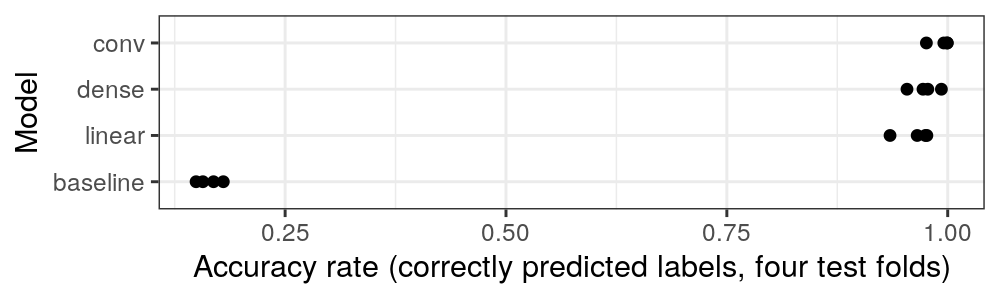
\includegraphics[width=\textwidth]{figure-test-accuracy-baseline}

  \begin{itemize}
  \item Always a good idea to compare with the trivial/featureless baseline model which always
    predicts the most frequent class in the train set. (ignoring all
    inputs/features) 
  \item Here we see that the featureless baseline is much less accurate than the
    three learned models, which are clearly learning something non-trivial.
  \item Code for test accuracy figures:
    \url{https://github.com/tdhock/2023-res-baz-az/blob/main/figure-test-accuracy.R}
  \end{itemize}
\end{frame}
 
\begin{frame}
  \frametitle{Zoom to learned models}
  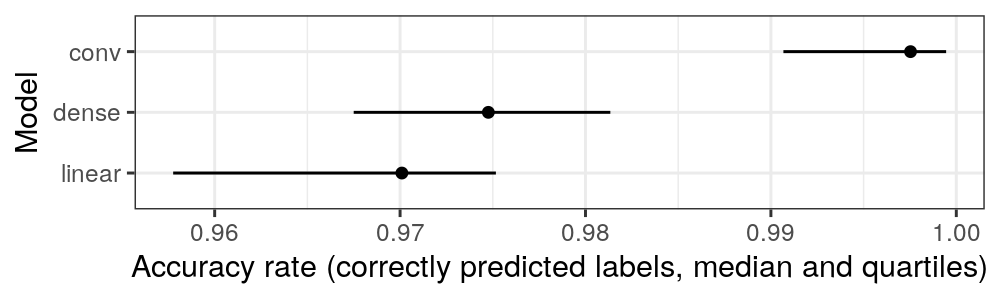
\includegraphics[width=\textwidth]{figure-test-accuracy}
  \begin{itemize}
  \item Dense neural network slightly more accurate
    than linear model, convolutional significantly more
    accurate than others.
  \item Conclusion: convolutional neural network should be preferred
    for most accurate predictions in these data.
  \item Maybe not the same conclusion in other data sets, with the
    same models. (always need to do cross-validation experiments to
    see which model is best in any given data set)
  \item Maybe other models/algorithms would be even more accurate in
    these data. (more/less layers, more/less units, completely
    different algorithm such as random forests, boosting, etc)
  \end{itemize}
\end{frame}

\section{Summary and quiz questions}

\begin{frame}
  \frametitle{Summary}
  Thanks for participating! We have studied
  \begin{itemize}
  \item Two kinds of machine learning problems, regression y=real number,
    classification y=integer category.
  \item Splitting a data set into train/test/subtrain/validation sets
    for learning hyper-parameters and evaluating prediction accuracy.
  \item Overfitting and how to avoid it by choosing hyper-parameters
    based on a validation set.
  \item Comparing prediction accuracy of learning algorithms with each
    other and to a featureless baseline.
  \end{itemize}
\end{frame}

\begin{frame}
  \frametitle{Quiz questions}
  \begin{itemize}
\item When using a design matrix to represent machine learning inputs,
  what does each row and column represent?
\item When splitting data into train/test sets, what is the purpose of
  each set? When splitting a train set into subtrain/validation sets,
  what is the purpose of each set?
\item In order to determine if any non-trivial predictive relationship
  between inputs and output has been learned, a comparison with a
  featureless baseline that ignores the inputs must be used. How do you compute
  the baseline predictions, for regression and classification
  problems?
\item How can you tell if machine learning model predictions are
  underfitting or overfitting?
\item Many learning algorithms require input of the number of
  iterations or epochs. For example in R the \texttt{nnet} function
  has the \texttt{maxit} argument and the \text{keras::fit} function
  has the \texttt{epochs} argument. How should this parameter be
  chosen?
  \end{itemize}
\end{frame}
 
\end{document}
